\documentclass[aps,prl,a4paper,superscriptaddress,twocolumn,showpacs,amsmath,amssymb,longbibliography]{revtex4-2} 


\usepackage{graphicx,epsfig}
\usepackage[usenames]{color}

\usepackage[english]{babel}

\DeclareMathOperator{\sgn}{sgn}


\usepackage{dsfont}


\usepackage{csquotes}
\MakeOuterQuote{"}


\setlength{\abovecaptionskip}{0pt} 

\allowdisplaybreaks


\begin{document}


\newcommand{\E}{\mathcal{E}}
\newcommand{\G}{\mathcal{G}}
\newcommand{\Lag}{\mathcal{L}}
\newcommand{\M}{\mathcal{M}}
\newcommand{\N}{\mathcal{N}}
\newcommand{\U}{\mathcal{U}}
\newcommand{\R}{\mathcal{R}}
\newcommand{\F}{\mathcal{F}}
\newcommand{\V}{\mathcal{V}}
\newcommand{\C}{\mathcal{C}}
\newcommand{\I}{\mathcal{I}}
\newcommand{\s}{\sigma}
\newcommand{\up}{\uparrow}
\newcommand{\dw}{\downarrow}
\newcommand{\h}{\hat{\mathcal{H}}}
\newcommand{\himp}{\hat{h}}
\newcommand{\g}{\mathcal{G}^{-1}_0}
\newcommand{\D}{\mathcal{D}}
\newcommand{\A}{\mathcal{A}}
\newcommand{\projs}{\hat{\mathcal{S}}_d}
\newcommand{\proj}{\hat{\mathcal{P}}_d}
\newcommand{\K}{\textbf{k}}
\newcommand{\Q}{\textbf{q}}
\newcommand{\T}{\tau_{\ast}}
\newcommand{\io}{i\omega_n}
\newcommand{\eps}{\varepsilon}
\newcommand{\+}{\dag}
\newcommand{\su}{\uparrow}
\newcommand{\giu}{\downarrow}
\newcommand{\0}[1]{\textbf{#1}}
%
\newcommand{\ca}{c^{\phantom{\dagger}}}
\newcommand{\cc}{c^\dagger}

\newcommand{\pa}{{p}^{\phantom{\dagger}}}
\newcommand{\pc}{{p}^\dagger}

\newcommand{\fa}{f^{\phantom{\dagger}}}
\newcommand{\fc}{f^\dagger}
%\newcommand{\ffa}{\hat{d}^{\phantom{\dagger}}}
%\newcommand{\ffc}{\hat{d}^\dagger}
%\newcommand{\fa}{\hat{f}^{\phantom{\dagger}}}
%\newcommand{\fc}{\hat{f}^\dagger}
%
\newcommand{\aaa}{a^{\phantom{\dagger}}}
\newcommand{\aac}{a^\dagger}
\newcommand{\bba}{b^{\phantom{\dagger}}}
\newcommand{\bbc}{b^\dagger}
\newcommand{\da}{{d}^{\phantom{\dagger}}}
\newcommand{\dc}{{d}^\dagger}
\newcommand{\ha}{h^{\phantom{\dagger}}}
\newcommand{\hc}{h^\dagger}
\newcommand{\be}{\begin{equation}}
\newcommand{\ee}{\end{equation}}
\newcommand{\bea}{\begin{eqnarray}}
\newcommand{\eea}{\end{eqnarray}}
\newcommand{\ba}{\begin{eqnarray*}}
\newcommand{\ea}{\end{eqnarray*}}
\newcommand{\dagga}{{\phantom{\dagger}}}
\newcommand{\bR}{\mathbf{R}}
\newcommand{\bQ}{\mathbf{Q}}
\newcommand{\bq}{\mathbf{q}}
\newcommand{\bqp}{\mathbf{q'}}
\newcommand{\bk}{\mathbf{k}}
\newcommand{\bh}{\mathbf{h}}
\newcommand{\bkp}{\mathbf{k'}}
\newcommand{\bp}{\mathbf{p}}
\newcommand{\bL}{\mathbf{L}}
\newcommand{\bRp}{\mathbf{R'}}
\newcommand{\bx}{\mathbf{x}}
\newcommand{\by}{\mathbf{y}}
\newcommand{\bz}{\mathbf{z}}
\newcommand{\br}{\mathbf{r}}
\newcommand{\Ima}{{\Im m}}
\newcommand{\Rea}{{\Re e}}
\newcommand{\Pj}[2]{|#1\rangle\langle #2|}
\newcommand{\ket}[1]{\vert#1\rangle}
\newcommand{\bra}[1]{\langle#1\vert}
\newcommand{\setof}[1]{\left\{#1\right\}}
\newcommand{\fract}[2]{\frac{\displaystyle #1}{\displaystyle #2}}
\newcommand{\Av}[2]{\langle #1|\,#2\,|#1\rangle}
\newcommand{\av}[1]{\langle #1 \rangle}
\newcommand{\Mel}[3]{\langle #1|#2\,|#3\rangle}
\newcommand{\Avs}[1]{\langle \,#1\,\rangle_0}
\newcommand{\eqn}[1]{(\ref{#1})}
\newcommand{\Tr}{\mathrm{Tr}}

\newcommand{\Vb}{\bar{\mathcal{V}}}
\newcommand{\Vd}{\Delta\mathcal{V}}
\def\P{P_{02}}
\newcommand{\Pb}{\bar{P}_{02}}
\newcommand{\Pd}{\Delta P_{02}}
\def\t{\theta_{02}}
\newcommand{\tb}{\bar{\theta}_{02}}
\newcommand{\td}{\Delta \theta_{02}}
\newcommand{\Rb}{\bar{R}}
\newcommand{\Rd}{\Delta R}
\newcommand{\ocrev}[1]{{\color{cyan}{#1}}}
\newcommand{\occom}[1]{{\color{red}{#1}}}



\title{Quantum-embedding description of the Anderson lattice model with \\ the ghost Gutzwiller Approximation}




\author{Marius S. Frank}
\affiliation{Department of Physics and Astronomy, Aarhus University, 8000, Aarhus C, Denmark}
\author{Tsung-Han Lee}
\affiliation{Physics and Astronomy Department, Rutgers University, Piscataway, New Jersey 08854, USA}
\author{Gargee Bhattacharyya}
\affiliation{Department of Physics and Astronomy, Aarhus University, 8000, Aarhus C, Denmark}
\author{Pak Ki Henry Tsang}
\affiliation{Department of Physics and National High Magnetic Field Laboratory, Florida State University, Tallahassee, Florida 32306, USA}
\author{Victor L. Quito}
\affiliation{Department of Physics and Astronomy, Iowa State University, Ames, Iowa 50011, USA}
\affiliation{Department of Physics and National High Magnetic Field Laboratory, Florida State University, Tallahassee, Florida 32306, USA}
\author{Vladimir Dobrosavljevi\'c}
\affiliation{Department of Physics and National High Magnetic Field Laboratory, Florida State University, Tallahassee, Florida 32306, USA}
\author{Ove Christiansen}
\affiliation{Department of Chemistry, Aarhus University, 8000, Aarhus C, Denmark}
\author{Nicola Lanat\`a}
\altaffiliation{Corresponding author: lanata@phys.au.dk}
\affiliation{Department of Physics and Astronomy, Aarhus University, 8000, Aarhus C, Denmark}
\affiliation{Nordita, KTH Royal Institute of Technology and Stockholm University, Hannes Alfv\'ens v\"ag 12, SE-106 91 Stockholm, Sweden}



\date{\today} 



\begin{abstract}

We present benchmark calculations of the Anderson lattice model based on the recently-developed "ghost Gutzwiller approximation".
%
%Our analysis shows that , while for the Hubbard model the standard Gutzwiller approximation (GA) provides us with a relatively accurate description of the Mott transition ---with a critical Hubbard interaction strength overestimated by only $\sim 10\%$ with respect to dynamical mean field theory (DMFT), ---  this is not the case for the ALM, where the metal-insulator transition can be incorrect by orders of magnitude.
%
Our analysis shows that, in some parameters regimes, the predictions of the standard Gutzwiller approximation can be incorrect by orders of magnitude for this model.
%
We show that this is caused by the inability of this method to describe simultaneously the Mott physics and the hybridization between correlated and itinerant degrees of freedom ---whose interplay often governs the metal-insulator transition in real materials.
%
Finally, we show that the ghost Gutzwiller approximation solves this problem, providing us with results in remarkable agreement with dynamical mean field theory throughout the entire phase diagram, while being much less computationally demanding.
%
We provide an analytical explanation of these findings and discuss
their implications within the context of ab-initio computation of strongly-correlated matter.

\end{abstract}






\maketitle


Understanding and simulating quantitatively the electronic behavior of strongly correlated matter is one of the most fundamental problems in condensed-matter science.
%
The substantial progress achieved today in this direction largely owes to quantum embedding methods~\cite{Kotliar-Science,quantum-embedding-review}.
%
In particular, the development of dynamical mean field theory (DMFT)~\cite{DMFT,dmft_book,CDMFT-Jarrell,CDMFT-Kotliar,CDMFT-Lichtenstein,CDMFT-Potthoff,CDMFT-Senechal,Aichhorn-DMFT-LAPW,LDA+U+DMFT,Held-review-DMFT,xidai_impl_LDA+DMFT} constituted a great leap in our understanding of strong-correlation phenomena, which advanced dramatically our ability of describing the properties of real materials.
%
In the past decade, the perspective of expanding the predictive power of simulations within the blooming field of theory-assisted materials-by-design~\cite{MaterialsGenome-1,MaterialsGenome-2} contributed to stimulate the development of alternative computational frameworks, capable of taking into account strong correlations at a lower computational cost.
%
Within this context, particularly promising approaches are the Gutzwiller approximation (GA)~\cite{Gutzwiller3,Fang,Ho,Bunemann-pnictides,Our-PRX,Gmethod} ---or, equivalently~\cite{equivalence_GA-SB,lanata-barone-fabrizio}, the rotationally-invariant slave-boson mean-field theory~\cite{Fresard1992,Georges,Lanata2016} --- and density matrix embedding theory~\cite{DMET,dmet-ghostcopy1}.
%
These frameworks have similar algorithmic structures. %and comparable accuracy. 
In fact, as in density matrix embedding theory, the GA equations can be cast in terms of ground-state calculations of auxiliary impurity models called embedding Hamiltonians (EH), where the bath has the same number of degrees of freedom as the impurity~\cite{Our-PRX}.
%
Furthermore, density matrix embedding theory can be formally derived from the GA equations, setting to unity the parameters encoding the quasiparticle mass-renormalization weights~\cite{dmet-risb-1,dmet-risb-2}.
%
More recently, a more accurate extension of the GA, called "ghost Gutzwiller approximation" (g-GA) has been developed~\cite{Ghost-GA}, based on the idea of extending the GA variational space introducing auxiliary (ghost) fermionic degrees of freedom.




Here we present benchmark calculations of the Anderson lattice model (ALM) and demonstrate that, by construction, the GA cannot capture the interplay between Mott physics and the hybridization between correlated and itinerant degrees of freedom ---which generally coexist and whose interplay often governs the metal-insulator transition in real materials. 
We also show that, in some parameters regimes, this limitation of the GA can result in overestimating the Mott critical point  by orders of magnitude.
%%(while, in the Hubbard model, the GA Mott point is only overestimated by $\sim 10\%$).
%
Finally, we demonstrate, both numerically and analytically, that the g-GA method resolves these problems, while remaining much less computationally demanding than DMFT.
%
Furthermore, we show that this method allows us to describe semi-analytically the spectral properties (both at low and high energies) throughout the entire phase diagram of the ALM, facilitating the physical interpretation of the numerical results.





%%%\section{Model}

\emph{Model}.--- 
We consider the ALM on a Bethe lattice, in the limit of infinite coordination number~\cite{GA-infinite-dim}:
\begin{align}
    \hat{H} &=  \sum_{<i,j>}\sum_{\sigma}  \left(t_{ij} + \delta_{ij}\epsilon_p\right)
   \pc_{i\sigma}\pa_{j\sigma} + \sum_{i}\frac{U}{2}\left(\hat{n}_{di}-1\right)^2 \nonumber\\
    &+ V\sum_{i\sigma}\left( \pc_{i\sigma}\da_{i\sigma} + \mathrm{H.c.}\right)
    - \mu\sum_i\hat{N}_i
    \nonumber
    \\
    &=
  \sum_{k\sigma}\sum_{\alpha\beta}[\tau_k]_{\alpha\beta}
  \,
  [\phi^\dagger_{k\sigma}]^\dagga_\alpha [\phi^\dagga_{k\sigma}]^\dagga_\beta
    +U\sum_i\dc_{i\uparrow}\da_{i\uparrow} \dc_{i\downarrow}\da_{i\downarrow}\,,
\end{align}
where:
$\pa_{i\sigma}$ and $\da_{i\sigma}$ are Fermionic annihilation operators, $\pc_{i\sigma}$ and $\dc_{i\sigma}$ are Fermionic creation operators, 
$i$ and $j$ are site labels, $\sigma$ is the spin, 
$<i,j>$ indicates that the corresponding summation is restricted to first nearest neighbours,
the hopping matrix $t_{ij}$ is uniform,
$\mu$ is the chemical potential,
$\hat{n}_{di}=\sum_{\sigma}\dc_{i\sigma}\da_{i\sigma}$,
$\hat{n}_{pi}=\sum_{\sigma}\pc_{i\sigma}\pa_{i\sigma}$,
$\hat{N}_i=\hat{n}_{di}+\hat{n}_{pi}$, %and we introduced:
$\phi^\dagger_{k\sigma}=(\pc_{k\sigma},\dc_{k\sigma})$,
$\phi^\dagger_{k\sigma}=\sum_i \mathcal{U}_{ik} \phi^\dagger_{i\sigma}$,
\begin{align}
    \tau_{k}=
    \begin{pmatrix}
    \epsilon_k+\epsilon_p-\mu & V  \\
    V & -U/2-\mu
    \end{pmatrix}
    \,,
\end{align}
the columns of $\mathcal{U}$ are the eigenvectors of $t$ and $\epsilon_k$ are its eigenvalues. 
%
From now on we fix the hopping matrix $t$ by using the half-bandwidth of $\epsilon_k$ (corresponding to a semi-circular density of states) as the energy unit.







%%%\section{Method}

\emph{Method}.--- 
Here we summarize the algorithmic structure of the g-GA and the GA, pointing out the key differences between these two methods, from a quantum-embedding perspective~\cite{Ghost-GA,Our-PRX,Lanata2016}.
%
For simplicity, below we focus on the ALM introduced above, while the general theory for arbitrary multi-orbital systems is summarized in the supplemental material~\cite{supplemental_material}.
%
%
For both the g-GA and the GA, the solution is obtained by calculating recursively the \emph{ground state} of 2 auxiliary systems: (1) the so-called "quasiparticle Hamiltonian" (QPH) and (2) the "embedding Hamiltonian" (EH).

The EH can be expressed in the following form:
\begin{align}
    \h_{\text{emb}}^{\text{g-GA}}&=
    \frac{U}{2}\left(\hat{n}_{d}-1\right)^2 -\mu\,\hat{n}_{d}
    +\sum_{\sigma}\sum_{a,b=1}^B\lambda^{\mathrm{c}}_{ab}\, \hat{f}^{\phantom{\dagger}}_{b\sigma}\hat{f}^{\dagger}_{a\sigma} 
    \nonumber\\
    &+\sum_{a=1}^B\sum_{\sigma}D_a \left( \hat{d}^{\dagger}_{\sigma}\hat{f}^{\phantom{\dagger}}_{a\sigma}+\mathrm{H.c.}\right) 
    \\
    \h_{\text{emb}}^{\text{GA}}&=
    \frac{U}{2}\left(\hat{n}_{d}-1\right)^2 -\mu\,\hat{n}_{d}
    + \sum_{\sigma}\lambda^c\, \hat{f}^{\phantom{\dagger}}_{\sigma}\hat{f}^{\dagger}_{\sigma}
    \nonumber\\
    &+\sum_{\sigma} D\left( \hat{d}^{\dagger}_{\sigma}\hat{f}^{\phantom{\dagger}}_{\sigma}+\mathrm{H.c.}\right)
    \,,
\end{align}
where the $\hat{d}$ operators correspond to the EH impurity degrees of freedom, $\hat{n}_{d}=\sum_{\sigma}\hat{d}^\dagger_{\sigma}\hat{d}^\dagga_{\sigma}$,
the $\hat{f}$ operators correspond to the EH bath degrees of freedom
and the parameters $D$ and $\lambda^c$ are determined self-consistently~\cite{supplemental_material}.
%
Note that, 
while in standard GA the bath of the EH has the same size of the impurity,
within the g-GA it contains a larger number of sites ($B>1$).
As in Refs.~\cite{Ghost-GA,exciton-mott-gga}, here we will set $B=3$
(the effect of increasing $B$, which would enlarge further the variational space, will be subject of future work).
%
After convergence, the expectation value of any local operator 
$\hat{O}[\dc_{i\alpha},\da_{i\alpha}]$ can be calculated from the
ground state $\ket{\Phi}$ of the EH as:
\be
\langle \hat{O} \rangle 
= \Av{\Phi}{\hat{O}[\hat{d}^{\dagger}_{\alpha},\hat{d}^{\dagga}_{\alpha}]}
\,.
\ee

The QPH can be expressed as:
\begin{align}
   \h_{\text{qp}}^{\text{g-GA}}&= \sum_{i\sigma}\sum_{a=1}^B l_a \fc_{ia\sigma}\fa_{ia\sigma} \nonumber\\
    &+ \sum_{i\sigma}\sum_{a=1}^B V\big(r_a \fc_{ia\sigma}\pa_{i\sigma} + \mathrm{H.c.}\big)\nonumber\\
    &+\sum_{i\sigma}\left(\epsilon_p-\mu\right) \pc_{i\sigma}\pa_{i\sigma}
    +\sum_{ij\sigma} t_{ij}\pc_{i\sigma}\pa_{j\sigma}
    \label{hqp-gga}
    \\
    \h_{\text{qp}}^{\text{GA}} &= \sum_{i\sigma}l\, \fc_{i\sigma}\fa_{i\sigma} + \sum_{i\sigma}V\big(r \fc_{i\sigma}\pa_{i\sigma} + \mathrm{H.c.}\big)\nonumber\\
    &+\sum_{i\sigma}\left(\epsilon_p-\mu\right) \pc_{i\sigma}\pa_{i\sigma}
    +\sum_{ij\sigma}t_{ij}\pc_{i\sigma}\pa_{j\sigma}
    \label{hqp-ga}
    \,,
\end{align}
where the $f_{ia\sigma}$ operators are "quasiparticle modes" residing in an auxiliary (enlarged) Hilbert space~\cite{supplemental_material}.
%
Once the parameters $l$ and $r$ are determined self-consistently in the form above~\cite{supplemental_material}, the resulting Green's function for the modes $\phi_{k\sigma}$ is:
\begin{align}
    \mathcal{G}(k,\omega)=\big[
    \omega-\tau_k-\Sigma(\omega)
    \big]^{-1}
    \,,
\end{align}
where the only non-zero entry of $\Sigma(\omega)$ is the $dd$ component, which is given by the following equations:
%%%%%%%
\begin{widetext}
\begin{align}
    \Sigma^{\text{g-GA}}_{dd}(\omega)&=
    \mu \! + \! \frac{U}{2} \! 
    + \! \frac{l_1}{r_1^2}
    \!-\! \omega\frac{1\!-\!r_1^2}{r_1^2}
    \!+\!\frac{(\omega\!-\!l_1)^2}{r_1^4}
    \big[
   (\omega\!-\!l_3)r_2^2+(\omega\!-\!l_2)r_3^2
    \big]
   \!\left[
    (\omega\!-\!l_2)(\omega\!-\!l_3)\!+\!\frac{\omega\!-\!l_1}{r_1^2}
    \big(
    r_2^2(\omega\!-\!l_3)\!+\!r_3^2(\omega\!-\!l_2)
    \big)
    \right]^{-1}
    \label{sigma-gga}
    \\
    \Sigma^{\text{GA}}_{dd}(\omega)&=
    \mu  + \frac{U}{2}
    + \frac{l}{r^2} - \omega\frac{1-r^2}{r^2}
    \label{sigma-ga}
    \,.
\end{align}
\end{widetext}


As demonstrated in the supplemental material~\cite{supplemental_material} (and shown in the calculations below): (i) the poles of
$\mathcal{G}(k,\omega)$ are located on top of the eigenvalues of the corresponding QPHs~\cite{hiddenQP-1,hiddenQP-2,hiddenQP-3,hiddenQP-4}, and
%
(ii) the resulting total spectral weight of the $d$ degrees of freedom is given by:
\begin{align}
    \int_{-\infty}^{\infty}
    \mathcal{A}^{\text{g-GA}}_{dd}(k,\omega)d\omega
    &=\sum_{a=1}^B r_a^2
    \label{totweight-gga}
    \\
    \int_{-\infty}^{\infty}
    \mathcal{A}^{\text{GA}}_{dd}(k,\omega)d\omega
    &=r^2
    \label{totweight-ga}
    \,,
\end{align}
where $\mathcal{A}^{\text{g-GA}}_{dd}$ and $\mathcal{A}^{\text{GA}}_{dd}$ are the g-GA and GA $d$-electron spectral functions, respectively, and $r^2$ is the GA $d$-electron quasiparticle weight~\cite{Gebhard-FL}.
%
%
From the parameters $R,\lambda$ and the ground state $\ket{\Psi_0}$ of the corresponding QPH,
it is also possible to calculate the expectation values of all non-local quadratic operators.
%
In particular:
\begin{align}
    \langle
    \dc_{i\sigma}\pa_{i\sigma}
    \rangle_{\text{g-GA}}
    &=\sum_{a=1}^B r_a 
    \Av{\Psi_0}{\fc_{ia\sigma}\pa_{i\sigma}}
    \label{hibr-gga}
    \\
    \langle
    \dc_{i\sigma}\pa_{i\sigma}
    \rangle_{\text{GA}}
    &=r 
    \Av{\Psi_0}{\fc_{i\sigma}\pa_{i\sigma}}
    \label{hibr-ga}
\,.
\end{align}



%Note that Eqs.~\eqref{sigma-gga}-\eqref{totweight-ga} are valid for generic single-orbital impurities.
%
For completeness, the generalization of all analytical results listed above to arbitrary multi-orbital systems is given in the supplemental material~\cite{supplemental_material}.



%%%\section{Results}


\begin{figure} %[htp]
    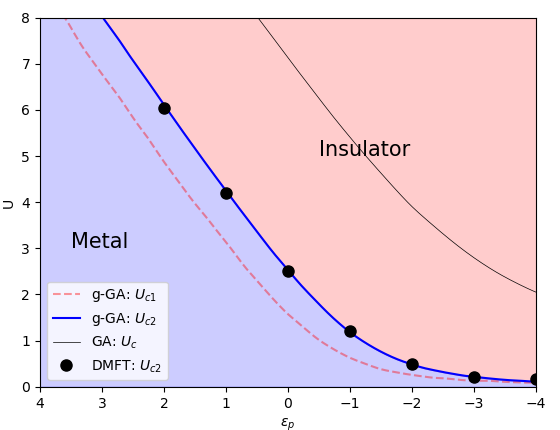
\includegraphics[width=8.7cm]{Figure1.png}
    \caption{Paramagnetic
    phase diagram of the ALM on an infinite-coordination Bethe lattice, for $3$ electrons per site and $V=1$.
    %
    The g-GA metal-insulator transition $U_{c2}$ and the end of the metal-insulator coexistence region $U_{c1}$ are marked in blue and red, respectively.
    %
    The black dots are $U_{c2}$ values calculated with DMFT+CTQMC, at $T=0.01$.
    %
    The gray line indicates the metal-insulator transition in bare GA.
    }
    \label{Figure1}
\end{figure}


\begin{figure*}[ht]
\begin{center}
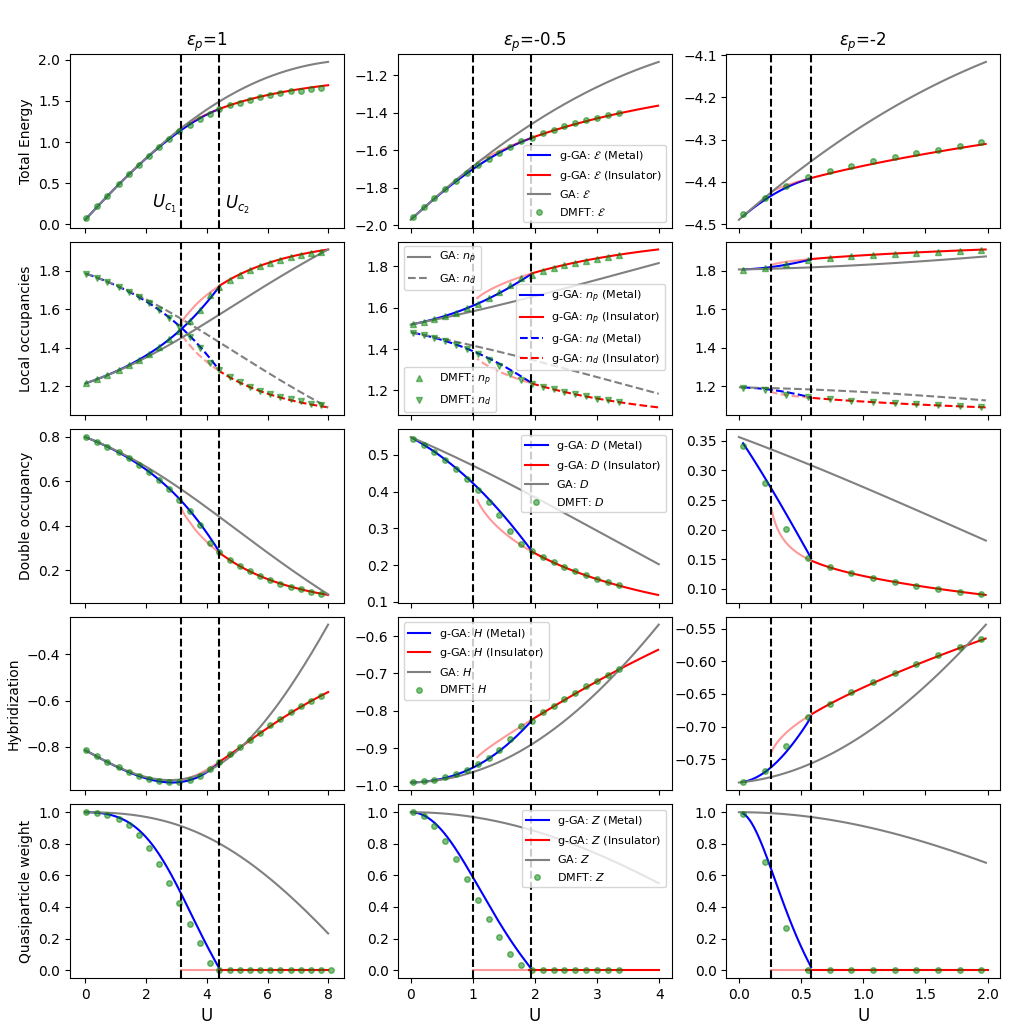
\includegraphics[width=17.5cm]{Figure2.png}
\caption{
Behavior of the g-GA total energy $\mathcal{E}$, local occupancies $n_p=\langle\hat{n}_{pi}\rangle$ and $n_d=\langle\hat{n}_{di}\rangle$, $d$-electron double occupancy
$D=\langle\hat{n}_{di\uparrow}\hat{n}_{di \downarrow}\rangle$,
$p$-$d$ hybridization $H=\sum_\sigma\langle
    \dc_{i\sigma} p_{i\sigma}
    \rangle +\text{c.c.}$
and $d$-electron quasiparticle weight $Z$,
%
for the ALM on an infinite-coordination Bethe lattice, in comparison with DMFT and the bare GA.
%
The DMFT data are computed with CTQMC, at $T=0.01$ for $\epsilon_p=1$ and $\epsilon_p=-0.5$ and at $T=0.02$ for $\epsilon_p=-2$.
The vertical black dashed lines indicate $U_{c1}$ and $U_{c2}$.
}
\label{Figure2}
\end{center}
\end{figure*}


\emph{Results}.--- 
In Fig.~\ref{Figure1} we show the g-GA phase diagram of the ALM
(in the paramagnetic phase) for total occupancy $\langle \hat{N}_{i}\rangle=3$.
%
The g-GA results are compared with DMFT ---with the continuous time quantum Monte Carlo (CTQMC) impurity solver~\cite{ctqmc,ctqmc-Gull-RevModPhys,ctqmc-Haule}, at temperature $T=0.01$--- and with the bare GA.
%%%
%%%The g-GA metal-insulator transition line $U_{c2}$ is marked in blue, the line indicating the end of the metal-insulator coexistence region $U_{c1}$ is marked in red and the DMFT $U_{c2}$ points are indicated by black dots.
%
Our benchmark calculations show that the g-GA phase diagram is consistent with previous work~\cite{ALM-1,ALM-2,ALM-3} and in remarkable agreement with DMFT.
%
As expected, both the g-GA method and the bare GA capture the fact that the Mott metal-insulator transition point $U_{c2}$ vanishes for $\eps_p\rightarrow -\infty$ ---corresponding to the limit where the $p$ degrees of freedom are gapped out.
%
However, the interaction $U_c$ of the metal-insulator transition 
%(marked by a thin gray line) 
is largely overestimated within the GA, especially for $\epsilon_p\ll -1$.
%
Note that the phase diagram for $\langle \hat{N}_{i}\rangle=1$ can be automatically inferred from our calculations above, as they are related to each other by a particle-hole transformation.


In Fig.~\ref{Figure2} we show the behavior of the g-GA total energy $\mathcal{E}$, the occupancies $n_p=\langle\hat{n}_{pi}\rangle$ and $n_d=\langle\hat{n}_{di}\rangle$, the $d$-electron double occupancy
$D=\langle\hat{n}_{di\uparrow}\hat{n}_{di \downarrow}\rangle$,
the $p$-$d$ "hybridization energy"
$H=\sum_\sigma\langle \dc_{i\sigma}\pa_{i\sigma} \rangle +\text{c.c.}$,
and the $d$-electron quasiparticle weight:
\begin{align}
    Z &= \left[ 1 - \frac{\partial \Sigma^{\mathrm{g-GA}}}{\partial\omega}\right]^{-1}_{\omega= 0}
    \nonumber
    \\
    &= \frac{\left(l_2 \, l_3 \, r_1^2 + l_1 \, l_3 \, r_2^2 + l_1 \, l_2 \, r_3^2\right)^2}
    {l_1^2 \, l_3^2 \, r_2^2 + l_2^2 \left(l_3^2 \, r_1^2 + l_1^2 \, r_3^2\right)}  
    %\\
    %Z^{\mathrm{GA}} &= r^2
    \,.
\end{align}
%
The g-GA results are shown in comparison with the bare GA and DMFT.
%
While the GA solution is considered accurate only for weak interactions, we find that the agreement between g-GA and DMFT is remarkable for all observables, in all parameters regimes.

\begin{figure*}[ht]
\begin{center}
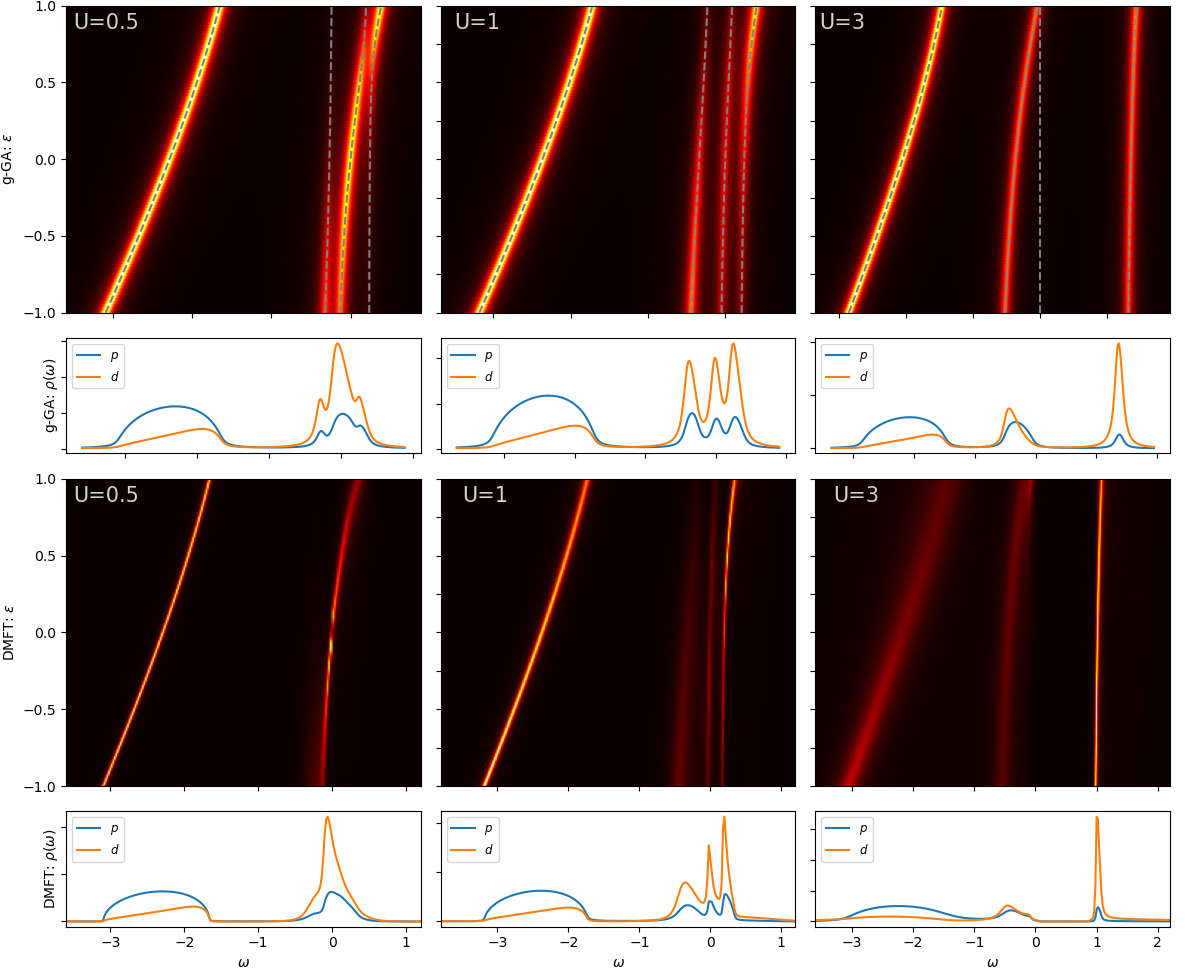
\includegraphics[width=17.5cm]{Figure3.png}
\caption{
Energy-resolved spectral function and corresponding $p$ and $d$ local density of states $\rho(\omega)$, calculated
with g-GA (upper panels) and DMFT+CTQMC (lower panels), for $\epsilon_p=-1$ and 3 values of $U$.
The g-GA spectra is visualized using a small artificial smearing, $\Gamma=0.06$.
The g-GA quasiparticle bands are indicated by gray dashed lines. 
}
\label{Figure3}
\end{center}
\end{figure*}


Let us now analyze the single-particle Green's function.
%
In Fig.~\ref{Figure3} we consider $\epsilon_p=-1$ and 3 values of $U$,
showing the total g-GA 
energy-resolved spectral function:
\be
\mathcal{A}(k,\omega)=-\frac{1}{\pi}\text{Im}
\Tr[\mathcal{G}(k,\omega)]
\ee
and the $p$ and $d$ local density of states.
%
The DMFT spectra were obtained by performing analytical continuation with the maximum entropy method~\cite{JARRELL1996133}.
%
Interestingly, the g-GA captures systematically the main features of the DMFT spectra (including the Hubbard bands, and the hybridization between the $p$ and $d$ degrees of freedom).
%
%
Note that, to interpret the behavior of the g-GA spectra, it is possible to exploit its relation with the bands of the QPH [Eq.~\eqref{hqp-gga}], previously discussed in the methods section.
%
In particular, the relative position of the $p$ band with respect to the Fermi level is approximately encoded in the corresponding on-site energy
$\epsilon_p^*=\epsilon_p-\mu$, while the positions of the $d$-electron low-energy and high-energy excitations are approximately encoded in the variational parameters $l_a$ ($a=1,2,3$).
%







%%\section{Discussion}


A key fact emerging from our benchmark calculations is that the GA can overestimate $U_c$ dramatically (especially for $\epsilon_p\ll -1$), see Fig.~\ref{Figure1}.
%
To explain this result we note that, by construction, the GA Mott transition occurs when the quasiparticle weight $Z=r^2$ vanishes, see Eq.~\eqref{sigma-ga}.
Therefore, the corresponding approximation to the Mott phase is such that $\langle\dc_{i\sigma}\pa_{i\sigma}\rangle_{\text{GA}}=0$, see Eq.~\eqref{hibr-ga}.
In other words, this method cannot describe simultaneously the Mott phase and the $p$-$d$ charge fluctuations.
%
But this is unrealistic for the ALM, where the $p$-$d$ hybridization effects are generally very large, not only in the weakly-interacting regime, but also for $U\simeq U_{c2}$ and $U>U_{c2}$, see Figs.~\ref{Figure2},\ref{Figure3}.
%
Because of the variational principle, this results in a systematic overestimation of the total energy as we approach the Mott phase (see Fig.~\ref{Figure2}), causing an overestimation of the metal-insulator transition point.
%
This point is documented in further detail in the supplemental material, where the GA overestimation of $U_{c}$ at $\epsilon_p\ll -1$ is explained in relation to a qualitative pathological behavior of the GA variational parameter $r$ in the narrow-bandwidth limit ($t\rightarrow 0)$. 


Remarkably, since the g-GA captures the existence of the Hubbard bands, the right side of Eq.~\eqref{totweight-gga} never vanishes~\cite{Ghost-GA}.
%
Therefore, similar to DMFT, $\langle\dc_{i\sigma}\pa_{i\sigma}\rangle_{\text{g-GA}}$
remains finite even in the Mott phase (see Eq.~\eqref{hibr-gga}).
%
This shows that the ability of the g-GA of describing simultaneously the Mott physics and the $d$-$p$ hybridization is directly connected with its ability of describing the transfer of $d$-electron spectral weight to the Hubbard bands (which the bare GA lacks).




%%%\section{Conclusions}

\emph{Conclusions}.--- 
We performed benchmark calculations of the ALM, showing that the g-GA provides us with results with accuracy comparable to DMFT, both for the ground-state and the spectral properties.
%
In particular, we showed that the g-GA is capable of describing accurately the interplay between the Mott physics and the hybridization between correlated and itinerant degrees of freedom, %%---which often governs the metal-insulator transition in real materials, --- 
while the GA cannot describe simultaneously these effects.
%
This is particularly relevant for real-material calculations in combination with density functional theory~\cite{Anisimov_DMFT,Fang,Our-PRX,LDA+U}, where the correlated orbitals are generally very localized around their atomic positions~\cite{Haule10,PWF2} ---so that the interactions with their environment are mainly mediated by the itinerant modes (as in the ALM studied here).
%
In fact, it is well possible that the limitation of the GA here uncovered explains why, in some cases, simulating the properties of real materials with the GA requires to use unphysically-large Hubbard $U$~\cite{npj-lanata}, and suggests that multi-orbital implementations of the g-GA will resolve these problems.


From the computational standpoint, the g-GA is more expensive than the bare GA (as the bath of the EH contains additional degrees of freedom). On the other hand, its 
computational complexity remains much lower than DMFT.
%
In fact, the g-GA requires to calculate only the ground state of a finite-size impurity model (while in DMFT it is necessary to calculate the spectra of an impurity model with an infinite bath).
%
For example, in our DMFT calculations each CTQMC iteration (performed using $5\times 10^8$ Monte Carlo steps, in parallel, on 72 cores) required about 2 minutes of computational time. Instead, within our g-GA calculations each EH iteration (performed on a single core) required about 0.2-0.3 seconds.
%
Note also that the difference in computational complexity between DMFT and g-GA grows exponentially as a function of the impurity size.


A particularly promising perspective is the possibility of solving the g-GA equations with hybrid quantum-classical frameworks~\cite{YY-qc}, employing impurity solvers based on quantum algorithms such as variational quantum eigensolvers~\cite{mcclean2016theory, o2016scalable, kandala2017hardware, romero2018strategies}.
%
In fact, within the g-GA, realizing such program for real-material applications may require devices consisting of only tens of qubits, while it has been estimated that quantum computers with at least 100 logical qubits will be necessary for applications within DMFT~\cite{HybridQC}.
%
Furthermore, since the number of parameters characterizing the EH is finite, the recently-developed approach based on machine learning for the GA~\cite{Our-ML-actinides} will be applicable also to the g-GA, as we hope to show in future work.
%%
Note also that the g-GA can be equivalently formulated in terms of the rotationally-invariant slave-boson mean-field theory~\cite{Ghost-GA}, which is based on an exact reformulation of the many-body problem. This line of interpretation may open the possibility of developing beyond-mean-field schemes, providing us with new routes for high-precision calculations.










\section*{Acknowledgements}
We thank Gabriel Kotliar for useful discussions.
%
We gratefully acknowledge funding from the Novo Nordisk Foundation through the Exploratory Interdisciplinary Synergy Programme project NNF19OC0057790.
%
We thank support from the VILLUM FONDEN through the Villum Experiment project 00028019 and the Centre of Excellence for Dirac Materials (Grant. No. 11744).
%
T.-H.L. was supported by the Computational Materials Sciences Program funded by the US Department of Energy, Office of Science, Basic
Energy Sciences, Materials Sciences and Engineering Division.
%
Work in Florida was supported by the NSF Grant No. 1822258, and the National High Magnetic Field Laboratory through the NSF Cooperative Agreement No. 1157490 and the State of Florida.









%%%\bibliography{ref}

%apsrev4-2.bst 2019-01-14 (MD) hand-edited version of apsrev4-1.bst
%Control: key (0)
%Control: author (8) initials jnrlst
%Control: editor formatted (1) identically to author
%Control: production of article title (0) allowed
%Control: page (0) single
%Control: year (1) truncated
%Control: production of eprint (0) enabled
\begin{thebibliography}{58}%
\makeatletter
\providecommand \@ifxundefined [1]{%
 \@ifx{#1\undefined}
}%
\providecommand \@ifnum [1]{%
 \ifnum #1\expandafter \@firstoftwo
 \else \expandafter \@secondoftwo
 \fi
}%
\providecommand \@ifx [1]{%
 \ifx #1\expandafter \@firstoftwo
 \else \expandafter \@secondoftwo
 \fi
}%
\providecommand \natexlab [1]{#1}%
\providecommand \enquote  [1]{``#1''}%
\providecommand \bibnamefont  [1]{#1}%
\providecommand \bibfnamefont [1]{#1}%
\providecommand \citenamefont [1]{#1}%
\providecommand \href@noop [0]{\@secondoftwo}%
\providecommand \href [0]{\begingroup \@sanitize@url \@href}%
\providecommand \@href[1]{\@@startlink{#1}\@@href}%
\providecommand \@@href[1]{\endgroup#1\@@endlink}%
\providecommand \@sanitize@url [0]{\catcode `\\12\catcode `\$12\catcode
  `\&12\catcode `\#12\catcode `\^12\catcode `\_12\catcode `\%12\relax}%
\providecommand \@@startlink[1]{}%
\providecommand \@@endlink[0]{}%
\providecommand \url  [0]{\begingroup\@sanitize@url \@url }%
\providecommand \@url [1]{\endgroup\@href {#1}{\urlprefix }}%
\providecommand \urlprefix  [0]{URL }%
\providecommand \Eprint [0]{\href }%
\providecommand \doibase [0]{https://doi.org/}%
\providecommand \selectlanguage [0]{\@gobble}%
\providecommand \bibinfo  [0]{\@secondoftwo}%
\providecommand \bibfield  [0]{\@secondoftwo}%
\providecommand \translation [1]{[#1]}%
\providecommand \BibitemOpen [0]{}%
\providecommand \bibitemStop [0]{}%
\providecommand \bibitemNoStop [0]{.\EOS\space}%
\providecommand \EOS [0]{\spacefactor3000\relax}%
\providecommand \BibitemShut  [1]{\csname bibitem#1\endcsname}%
\let\auto@bib@innerbib\@empty
%</preamble>
\bibitem [{\citenamefont {Kent}\ and\ \citenamefont
  {Kotliar}(2018)}]{Kotliar-Science}%
  \BibitemOpen
  \bibfield  {author} {\bibinfo {author} {\bibfnamefont {P.~R.~C.}\
  \bibnamefont {Kent}}\ and\ \bibinfo {author} {\bibfnamefont {G.}~\bibnamefont
  {Kotliar}},\ }\bibfield  {title} {\bibinfo {title} {Toward a predictive
  theory of correlated materials},\ }\href
  {https://doi.org/10.1126/science.aat5975} {\bibfield  {journal} {\bibinfo
  {journal} {Science}\ }\textbf {\bibinfo {volume} {361}},\ \bibinfo {pages}
  {348} (\bibinfo {year} {2018})}\BibitemShut {NoStop}%
\bibitem [{\citenamefont {Sun}\ and\ \citenamefont
  {Chan}(2016)}]{quantum-embedding-review}%
  \BibitemOpen
  \bibfield  {author} {\bibinfo {author} {\bibfnamefont {Q.}~\bibnamefont
  {Sun}}\ and\ \bibinfo {author} {\bibfnamefont {G.-K.-L.}\ \bibnamefont
  {Chan}},\ }\bibfield  {title} {\bibinfo {title} {Quantum embedding
  theories},\ }\href@noop {} {\bibfield  {journal} {\bibinfo  {journal} {Acc.
  Chem. Res.}\ }\textbf {\bibinfo {volume} {49}},\ \bibinfo {pages} {2705}
  (\bibinfo {year} {2016})}\BibitemShut {NoStop}%
\bibitem [{\citenamefont {Georges}\ \emph {et~al.}(1996)\citenamefont
  {Georges}, \citenamefont {Kotliar}, \citenamefont {Krauth},\ and\
  \citenamefont {Rozenberg}}]{DMFT}%
  \BibitemOpen
  \bibfield  {author} {\bibinfo {author} {\bibfnamefont {A.}~\bibnamefont
  {Georges}}, \bibinfo {author} {\bibfnamefont {G.}~\bibnamefont {Kotliar}},
  \bibinfo {author} {\bibfnamefont {W.}~\bibnamefont {Krauth}},\ and\ \bibinfo
  {author} {\bibfnamefont {M.~J.}\ \bibnamefont {Rozenberg}},\ }\bibfield
  {title} {\bibinfo {title} {Dynamical mean-field theory of strongly correlated
  fermion systems and the limit of infinite dimensions},\ }\href@noop {}
  {\bibfield  {journal} {\bibinfo  {journal} {Rev. Mod. Phys.}\ }\textbf
  {\bibinfo {volume} {68}},\ \bibinfo {pages} {13} (\bibinfo {year}
  {1996})}\BibitemShut {NoStop}%
\bibitem [{\citenamefont {Anisimov}\ and\ \citenamefont
  {Izyumov}(2010)}]{dmft_book}%
  \BibitemOpen
  \bibfield  {author} {\bibinfo {author} {\bibfnamefont {V.}~\bibnamefont
  {Anisimov}}\ and\ \bibinfo {author} {\bibfnamefont {Y.}~\bibnamefont
  {Izyumov}},\ }\href@noop {} {\emph {\bibinfo {title} {Electronic Structure of
  Strongly Correlated Materials}}}\ (\bibinfo  {publisher} {Springer},\
  \bibinfo {year} {2010})\BibitemShut {NoStop}%
\bibitem [{\citenamefont {Maier}\ \emph {et~al.}(2005)\citenamefont {Maier},
  \citenamefont {Jarrell}, \citenamefont {Pruschke},\ and\ \citenamefont
  {Hettler}}]{CDMFT-Jarrell}%
  \BibitemOpen
  \bibfield  {author} {\bibinfo {author} {\bibfnamefont {T.}~\bibnamefont
  {Maier}}, \bibinfo {author} {\bibfnamefont {M.}~\bibnamefont {Jarrell}},
  \bibinfo {author} {\bibfnamefont {T.}~\bibnamefont {Pruschke}},\ and\
  \bibinfo {author} {\bibfnamefont {M.~H.}\ \bibnamefont {Hettler}},\
  }\bibfield  {title} {\bibinfo {title} {Quantum cluster theories},\
  }\href@noop {} {\bibfield  {journal} {\bibinfo  {journal} {Rev. Mod. Phys.}\
  }\textbf {\bibinfo {volume} {77}},\ \bibinfo {pages} {1027} (\bibinfo {year}
  {2005})}\BibitemShut {NoStop}%
\bibitem [{\citenamefont {Kotliar}\ \emph {et~al.}(2001)\citenamefont
  {Kotliar}, \citenamefont {Savrasov}, \citenamefont {P\'alsson},\ and\
  \citenamefont {Biroli}}]{CDMFT-Kotliar}%
  \BibitemOpen
  \bibfield  {author} {\bibinfo {author} {\bibfnamefont {G.}~\bibnamefont
  {Kotliar}}, \bibinfo {author} {\bibfnamefont {S.~Y.}\ \bibnamefont
  {Savrasov}}, \bibinfo {author} {\bibfnamefont {G.}~\bibnamefont
  {P\'alsson}},\ and\ \bibinfo {author} {\bibfnamefont {G.}~\bibnamefont
  {Biroli}},\ }\bibfield  {title} {\bibinfo {title} {Cellular dynamical mean
  field approach to strongly correlated systems},\ }\href@noop {} {\bibfield
  {journal} {\bibinfo  {journal} {Phys. Rev. Lett.}\ }\textbf {\bibinfo
  {volume} {87}},\ \bibinfo {pages} {186401} (\bibinfo {year}
  {2001})}\BibitemShut {NoStop}%
\bibitem [{\citenamefont {Lichtenstein}\ and\ \citenamefont
  {Katsnelson}(2000)}]{CDMFT-Lichtenstein}%
  \BibitemOpen
  \bibfield  {author} {\bibinfo {author} {\bibfnamefont {A.~I.}\ \bibnamefont
  {Lichtenstein}}\ and\ \bibinfo {author} {\bibfnamefont {M.~I.}\ \bibnamefont
  {Katsnelson}},\ }\bibfield  {title} {\bibinfo {title} {Antiferromagnetism and
  $d$-wave superconductivity in cuprates: A cluster dynamical mean-field
  theory},\ }\href@noop {} {\bibfield  {journal} {\bibinfo  {journal} {Phys.
  Rev. B}\ }\textbf {\bibinfo {volume} {62}},\ \bibinfo {pages} {R9283}
  (\bibinfo {year} {2000})}\BibitemShut {NoStop}%
\bibitem [{\citenamefont {Potthoff}\ \emph {et~al.}(2003)\citenamefont
  {Potthoff}, \citenamefont {Aichhorn},\ and\ \citenamefont
  {Dahnken}}]{CDMFT-Potthoff}%
  \BibitemOpen
  \bibfield  {author} {\bibinfo {author} {\bibfnamefont {M.}~\bibnamefont
  {Potthoff}}, \bibinfo {author} {\bibfnamefont {M.}~\bibnamefont {Aichhorn}},\
  and\ \bibinfo {author} {\bibfnamefont {C.}~\bibnamefont {Dahnken}},\
  }\bibfield  {title} {\bibinfo {title} {Variational cluster approach to
  correlated electron systems in low dimensions},\ }\href@noop {} {\bibfield
  {journal} {\bibinfo  {journal} {Phys. Rev. Lett.}\ }\textbf {\bibinfo
  {volume} {91}},\ \bibinfo {pages} {206402} (\bibinfo {year}
  {2003})}\BibitemShut {NoStop}%
\bibitem [{\citenamefont {Senechal}\ \emph {et~al.}(2000)\citenamefont
  {Senechal}, \citenamefont {Perez},\ and\ \citenamefont
  {Pioro-Ladriere}}]{CDMFT-Senechal}%
  \BibitemOpen
  \bibfield  {author} {\bibinfo {author} {\bibfnamefont {D.}~\bibnamefont
  {Senechal}}, \bibinfo {author} {\bibfnamefont {D.}~\bibnamefont {Perez}},\
  and\ \bibinfo {author} {\bibfnamefont {M.}~\bibnamefont {Pioro-Ladriere}},\
  }\bibfield  {title} {\bibinfo {title} {The spectral weight of the
  $\text{Hubbard}$ model through cluster perturbation theory},\ }\href@noop {}
  {\bibfield  {journal} {\bibinfo  {journal} {Phys. Rev. Lett.}\ }\textbf
  {\bibinfo {volume} {84}},\ \bibinfo {pages} {522} (\bibinfo {year}
  {2000})}\BibitemShut {NoStop}%
\bibitem [{\citenamefont {Aichhorn}\ \emph {et~al.}(2009)\citenamefont
  {Aichhorn}, \citenamefont {Pourovskii}, \citenamefont {Vildosola},
  \citenamefont {Ferrero}, \citenamefont {Parcollet}, \citenamefont {Miyake},
  \citenamefont {Georges},\ and\ \citenamefont
  {Biermann}}]{Aichhorn-DMFT-LAPW}%
  \BibitemOpen
  \bibfield  {author} {\bibinfo {author} {\bibfnamefont {M.}~\bibnamefont
  {Aichhorn}}, \bibinfo {author} {\bibfnamefont {L.}~\bibnamefont
  {Pourovskii}}, \bibinfo {author} {\bibfnamefont {V.}~\bibnamefont
  {Vildosola}}, \bibinfo {author} {\bibfnamefont {M.}~\bibnamefont {Ferrero}},
  \bibinfo {author} {\bibfnamefont {O.}~\bibnamefont {Parcollet}}, \bibinfo
  {author} {\bibfnamefont {T.}~\bibnamefont {Miyake}}, \bibinfo {author}
  {\bibfnamefont {A.}~\bibnamefont {Georges}},\ and\ \bibinfo {author}
  {\bibfnamefont {S.}~\bibnamefont {Biermann}},\ }\bibfield  {title} {\bibinfo
  {title} {Dynamical mean-field theory within an augmented plane-wave
  framework: Assessing electronic correlations in the iron pnictide
  $\text{LaFeAsO}$},\ }\href@noop {} {\bibfield  {journal} {\bibinfo  {journal}
  {Phys. Rev. B}\ }\textbf {\bibinfo {volume} {80}},\ \bibinfo {pages} {085101}
  (\bibinfo {year} {2009})}\BibitemShut {NoStop}%
\bibitem [{\citenamefont {Kotliar}\ \emph {et~al.}(2006)\citenamefont
  {Kotliar}, \citenamefont {Savrasov}, \citenamefont {Haule}, \citenamefont
  {Oudovenko}, \citenamefont {Parcollet},\ and\ \citenamefont
  {Marianetti}}]{LDA+U+DMFT}%
  \BibitemOpen
  \bibfield  {author} {\bibinfo {author} {\bibfnamefont {G.}~\bibnamefont
  {Kotliar}}, \bibinfo {author} {\bibfnamefont {S.~Y.}\ \bibnamefont
  {Savrasov}}, \bibinfo {author} {\bibfnamefont {K.}~\bibnamefont {Haule}},
  \bibinfo {author} {\bibfnamefont {V.~S.}\ \bibnamefont {Oudovenko}}, \bibinfo
  {author} {\bibfnamefont {O.}~\bibnamefont {Parcollet}},\ and\ \bibinfo
  {author} {\bibfnamefont {C.~A.}\ \bibnamefont {Marianetti}},\ }\bibfield
  {title} {\bibinfo {title} {Electronic structure calculations with dynamical
  mean-field theory},\ }\href@noop {} {\bibfield  {journal} {\bibinfo
  {journal} {Rev. Mod. Phys.}\ }\textbf {\bibinfo {volume} {78}},\ \bibinfo
  {eid} {865} (\bibinfo {year} {2006})}\BibitemShut {NoStop}%
\bibitem [{\citenamefont {Held}\ \emph {et~al.}(2006)\citenamefont {Held},
  \citenamefont {Nekrasov}, \citenamefont {Keller}, \citenamefont {Eyert},
  \citenamefont {Bl\"umer}, \citenamefont {McMahan}, \citenamefont {Scalettar},
  \citenamefont {Pruschke}, \citenamefont {Anisimov},\ and\ \citenamefont
  {Vollhardt}}]{Held-review-DMFT}%
  \BibitemOpen
  \bibfield  {author} {\bibinfo {author} {\bibfnamefont {K.}~\bibnamefont
  {Held}}, \bibinfo {author} {\bibfnamefont {A.}~\bibnamefont {Nekrasov}},
  \bibinfo {author} {\bibfnamefont {G.}~\bibnamefont {Keller}}, \bibinfo
  {author} {\bibfnamefont {V.}~\bibnamefont {Eyert}}, \bibinfo {author}
  {\bibfnamefont {N.}~\bibnamefont {Bl\"umer}}, \bibinfo {author}
  {\bibfnamefont {A.~K.}\ \bibnamefont {McMahan}}, \bibinfo {author}
  {\bibfnamefont {R.~T.}\ \bibnamefont {Scalettar}}, \bibinfo {author}
  {\bibfnamefont {T.}~\bibnamefont {Pruschke}}, \bibinfo {author}
  {\bibfnamefont {V.~I.}\ \bibnamefont {Anisimov}},\ and\ \bibinfo {author}
  {\bibfnamefont {D.}~\bibnamefont {Vollhardt}},\ }\bibfield  {title} {\bibinfo
  {title} {Realistic investigations of correlated electron systems with
  $\text{LDA+DMFT}$},\ }\href@noop {} {\bibfield  {journal} {\bibinfo
  {journal} {Phys. Stat. Sol. (B)}\ }\textbf {\bibinfo {volume} {243}},\
  \bibinfo {pages} {2599} (\bibinfo {year} {2006})}\BibitemShut {NoStop}%
\bibitem [{\citenamefont {Zhao}\ \emph {et~al.}(2012)\citenamefont {Zhao},
  \citenamefont {Zhuang}, \citenamefont {Deng}, \citenamefont {Bi},
  \citenamefont {Cai}, \citenamefont {Fang},\ and\ \citenamefont
  {Dai}}]{xidai_impl_LDA+DMFT}%
  \BibitemOpen
  \bibfield  {author} {\bibinfo {author} {\bibfnamefont {J.-Z.}\ \bibnamefont
  {Zhao}}, \bibinfo {author} {\bibfnamefont {J.-N.}\ \bibnamefont {Zhuang}},
  \bibinfo {author} {\bibfnamefont {X.-Y.}\ \bibnamefont {Deng}}, \bibinfo
  {author} {\bibfnamefont {Y.}~\bibnamefont {Bi}}, \bibinfo {author}
  {\bibfnamefont {L.-C.}\ \bibnamefont {Cai}}, \bibinfo {author} {\bibfnamefont
  {Z.}~\bibnamefont {Fang}},\ and\ \bibinfo {author} {\bibfnamefont
  {X.}~\bibnamefont {Dai}},\ }\bibfield  {title} {\bibinfo {title}
  {Implementation of $\text{LDA+DMFT}$ with the pseudo-potential-plane-wave
  method},\ }\href@noop {} {\bibfield  {journal} {\bibinfo  {journal} {Chin.
  Phys. B}\ }\textbf {\bibinfo {volume} {21}},\ \bibinfo {pages} {057106}
  (\bibinfo {year} {2012})}\BibitemShut {NoStop}%
\bibitem [{\citenamefont {Chen}\ \emph {et~al.}(2015)\citenamefont {Chen},
  \citenamefont {Chen}, \citenamefont {Kalinin}, \citenamefont {Klimeck},
  \citenamefont {Kumar}, \citenamefont {Neugebauer},\ and\ \citenamefont
  {Terasaki}}]{MaterialsGenome-1}%
  \BibitemOpen
  \bibfield  {author} {\bibinfo {author} {\bibfnamefont {L.-Q.}\ \bibnamefont
  {Chen}}, \bibinfo {author} {\bibfnamefont {L.-D.}\ \bibnamefont {Chen}},
  \bibinfo {author} {\bibfnamefont {S.~V.}\ \bibnamefont {Kalinin}}, \bibinfo
  {author} {\bibfnamefont {G.}~\bibnamefont {Klimeck}}, \bibinfo {author}
  {\bibfnamefont {S.~K.}\ \bibnamefont {Kumar}}, \bibinfo {author}
  {\bibfnamefont {J.}~\bibnamefont {Neugebauer}},\ and\ \bibinfo {author}
  {\bibfnamefont {I.}~\bibnamefont {Terasaki}},\ }\bibfield  {title} {\bibinfo
  {title} {Design and discovery of materials guided by theory and
  computation},\ }\href@noop {} {\bibfield  {journal} {\bibinfo  {journal} {npj
  Computational Materials}\ }\textbf {\bibinfo {volume} {1}},\ \bibinfo {pages}
  {15007} (\bibinfo {year} {2015})}\BibitemShut {NoStop}%
\bibitem [{\citenamefont {Adler}\ \emph {et~al.}(2018)\citenamefont {Adler},
  \citenamefont {Kang}, \citenamefont {Yee},\ and\ \citenamefont
  {Kotliar}}]{MaterialsGenome-2}%
  \BibitemOpen
  \bibfield  {author} {\bibinfo {author} {\bibfnamefont {R.}~\bibnamefont
  {Adler}}, \bibinfo {author} {\bibfnamefont {C.-J.}\ \bibnamefont {Kang}},
  \bibinfo {author} {\bibfnamefont {C.-H.}\ \bibnamefont {Yee}},\ and\ \bibinfo
  {author} {\bibfnamefont {G.}~\bibnamefont {Kotliar}},\ }\bibfield  {title}
  {\bibinfo {title} {Correlated materials design: prospects and challenges},\
  }\href@noop {} {\bibfield  {journal} {\bibinfo  {journal} {Reports on
  Progress in Physics}\ }\textbf {\bibinfo {volume} {82}},\ \bibinfo {pages}
  {012504} (\bibinfo {year} {2018})}\BibitemShut {NoStop}%
\bibitem [{\citenamefont {Gutzwiller}(1965)}]{Gutzwiller3}%
  \BibitemOpen
  \bibfield  {author} {\bibinfo {author} {\bibfnamefont {M.~C.}\ \bibnamefont
  {Gutzwiller}},\ }\bibfield  {title} {\bibinfo {title} {Correlation of
  {Electrons} in a {Narrow} {$s$} {Band}},\ }\href
  {https://doi.org/10.1103/PhysRev.137.A1726} {\bibfield  {journal} {\bibinfo
  {journal} {Phys. Rev.}\ }\textbf {\bibinfo {volume} {137}},\ \bibinfo {pages}
  {A1726} (\bibinfo {year} {1965})}\BibitemShut {NoStop}%
\bibitem [{\citenamefont {Deng}\ \emph {et~al.}(2009)\citenamefont {Deng},
  \citenamefont {Wang}, \citenamefont {Dai},\ and\ \citenamefont
  {Fang}}]{Fang}%
  \BibitemOpen
  \bibfield  {author} {\bibinfo {author} {\bibfnamefont {X.-Y.}\ \bibnamefont
  {Deng}}, \bibinfo {author} {\bibfnamefont {L.}~\bibnamefont {Wang}}, \bibinfo
  {author} {\bibfnamefont {X.}~\bibnamefont {Dai}},\ and\ \bibinfo {author}
  {\bibfnamefont {Z.}~\bibnamefont {Fang}},\ }\bibfield  {title} {\bibinfo
  {title} {Local density approximation combined with {Gutzwiller} method for
  correlated electron systems: {Formalism} and applications},\ }\href@noop {}
  {\bibfield  {journal} {\bibinfo  {journal} {Phys. Rev. B}\ }\textbf {\bibinfo
  {volume} {79}},\ \bibinfo {eid} {075114} (\bibinfo {year}
  {2009})}\BibitemShut {NoStop}%
\bibitem [{\citenamefont {Ho}\ \emph {et~al.}(2008)\citenamefont {Ho},
  \citenamefont {Schmalian},\ and\ \citenamefont {Wang}}]{Ho}%
  \BibitemOpen
  \bibfield  {author} {\bibinfo {author} {\bibfnamefont {K.~M.}\ \bibnamefont
  {Ho}}, \bibinfo {author} {\bibfnamefont {J.}~\bibnamefont {Schmalian}},\ and\
  \bibinfo {author} {\bibfnamefont {C.~Z.}\ \bibnamefont {Wang}},\ }\bibfield
  {title} {\bibinfo {title} {Gutzwiller density functional theory for
  correlated electron systems},\ }\href
  {https://doi.org/10.1103/PhysRevB.77.073101} {\bibfield  {journal} {\bibinfo
  {journal} {Phys. Rev. B}\ }\textbf {\bibinfo {volume} {77}},\ \bibinfo
  {pages} {073101} (\bibinfo {year} {2008})}\BibitemShut {NoStop}%
\bibitem [{\citenamefont {Schickling}\ \emph {et~al.}(2011)\citenamefont
  {Schickling}, \citenamefont {Gebhard},\ and\ \citenamefont
  {B\"unemann}}]{Bunemann-pnictides}%
  \BibitemOpen
  \bibfield  {author} {\bibinfo {author} {\bibfnamefont {T.}~\bibnamefont
  {Schickling}}, \bibinfo {author} {\bibfnamefont {F.}~\bibnamefont
  {Gebhard}},\ and\ \bibinfo {author} {\bibfnamefont {J.}~\bibnamefont
  {B\"unemann}},\ }\bibfield  {title} {\bibinfo {title} {Antiferromagnetic
  order in multiband $\text{Hubbard}$ models for iron pnictides},\ }\href@noop
  {} {\bibfield  {journal} {\bibinfo  {journal} {Phys. Rev. Lett.}\ }\textbf
  {\bibinfo {volume} {106}},\ \bibinfo {pages} {146402} (\bibinfo {year}
  {2011})}\BibitemShut {NoStop}%
\bibitem [{\citenamefont {Lanat\`a}\ \emph {et~al.}(2015)\citenamefont
  {Lanat\`a}, \citenamefont {Yao}, \citenamefont {Wang}, \citenamefont {Ho},\
  and\ \citenamefont {Kotliar}}]{Our-PRX}%
  \BibitemOpen
  \bibfield  {author} {\bibinfo {author} {\bibfnamefont {N.}~\bibnamefont
  {Lanat\`a}}, \bibinfo {author} {\bibfnamefont {Y.-X.}\ \bibnamefont {Yao}},
  \bibinfo {author} {\bibfnamefont {C.-Z.}\ \bibnamefont {Wang}}, \bibinfo
  {author} {\bibfnamefont {K.-M.}\ \bibnamefont {Ho}},\ and\ \bibinfo {author}
  {\bibfnamefont {G.}~\bibnamefont {Kotliar}},\ }\bibfield  {title} {\bibinfo
  {title} {Phase diagram and electronic structure of praseodymium and
  plutonium},\ }\href@noop {} {\bibfield  {journal} {\bibinfo  {journal} {Phys.
  Rev. X}\ }\textbf {\bibinfo {volume} {5}},\ \bibinfo {pages} {011008}
  (\bibinfo {year} {2015})}\BibitemShut {NoStop}%
\bibitem [{\citenamefont {Lanat\`a}\ \emph {et~al.}(2012)\citenamefont
  {Lanat\`a}, \citenamefont {Strand}, \citenamefont {Dai},\ and\ \citenamefont
  {Hellsing}}]{Gmethod}%
  \BibitemOpen
  \bibfield  {author} {\bibinfo {author} {\bibfnamefont {N.}~\bibnamefont
  {Lanat\`a}}, \bibinfo {author} {\bibfnamefont {H.~U.~R.}\ \bibnamefont
  {Strand}}, \bibinfo {author} {\bibfnamefont {X.}~\bibnamefont {Dai}},\ and\
  \bibinfo {author} {\bibfnamefont {B.}~\bibnamefont {Hellsing}},\ }\bibfield
  {title} {\bibinfo {title} {Efficient implementation of the
  $\text{Gutzwiller}$ variational method},\ }\href
  {https://doi.org/10.1103/PhysRevB.85.035133} {\bibfield  {journal} {\bibinfo
  {journal} {Phys. Rev. B}\ }\textbf {\bibinfo {volume} {85}},\ \bibinfo
  {pages} {035133} (\bibinfo {year} {2012})}\BibitemShut {NoStop}%
\bibitem [{\citenamefont {B\"unemann}\ and\ \citenamefont
  {Gebhard}(2007)}]{equivalence_GA-SB}%
  \BibitemOpen
  \bibfield  {author} {\bibinfo {author} {\bibfnamefont {J.}~\bibnamefont
  {B\"unemann}}\ and\ \bibinfo {author} {\bibfnamefont {F.}~\bibnamefont
  {Gebhard}},\ }\bibfield  {title} {\bibinfo {title} {Equivalence of
  $\text{Gutzwiller}$ and slave-boson mean-field theories for multiband
  $\text{Hubbard}$ models},\ }\href@noop {} {\bibfield  {journal} {\bibinfo
  {journal} {Phys. Rev. B}\ }\textbf {\bibinfo {volume} {76}},\ \bibinfo
  {pages} {193104} (\bibinfo {year} {2007})}\BibitemShut {NoStop}%
\bibitem [{\citenamefont {Lanat\`{a}}\ \emph {et~al.}(2008)\citenamefont
  {Lanat\`{a}}, \citenamefont {Barone},\ and\ \citenamefont
  {Fabrizio}}]{lanata-barone-fabrizio}%
  \BibitemOpen
  \bibfield  {author} {\bibinfo {author} {\bibfnamefont {N.}~\bibnamefont
  {Lanat\`{a}}}, \bibinfo {author} {\bibfnamefont {P.}~\bibnamefont {Barone}},\
  and\ \bibinfo {author} {\bibfnamefont {M.}~\bibnamefont {Fabrizio}},\
  }\bibfield  {title} {\bibinfo {title} {Fermi-surface evolution across the
  magnetic phase transition in the {Kondo} lattice model},\ }\href@noop {}
  {\bibfield  {journal} {\bibinfo  {journal} {Phys. Rev. B}\ }\textbf {\bibinfo
  {volume} {78}},\ \bibinfo {eid} {155127} (\bibinfo {year}
  {2008})}\BibitemShut {NoStop}%
\bibitem [{\citenamefont {Fr{\'{e}}sard}\ and\ \citenamefont
  {W{\"{o}}lfle}(1992)}]{Fresard1992}%
  \BibitemOpen
  \bibfield  {author} {\bibinfo {author} {\bibfnamefont {R.}~\bibnamefont
  {Fr{\'{e}}sard}}\ and\ \bibinfo {author} {\bibfnamefont {P.}~\bibnamefont
  {W{\"{o}}lfle}},\ }\bibfield  {title} {\bibinfo {title} {Unified slave boson
  representation of spin and charge degrees of freedom for strongly correlated
  fermi systems},\ }\href {https://doi.org/10.1142/S0217979292000414}
  {\bibfield  {journal} {\bibinfo  {journal} {International Journal of Modern
  Physics B}\ }\textbf {\bibinfo {volume} {06}},\ \bibinfo {pages} {685}
  (\bibinfo {year} {1992})}\BibitemShut {NoStop}%
\bibitem [{\citenamefont {Lechermann}\ \emph {et~al.}(2007)\citenamefont
  {Lechermann}, \citenamefont {Georges}, \citenamefont {Kotliar},\ and\
  \citenamefont {Parcollet}}]{Georges}%
  \BibitemOpen
  \bibfield  {author} {\bibinfo {author} {\bibfnamefont {F.}~\bibnamefont
  {Lechermann}}, \bibinfo {author} {\bibfnamefont {A.}~\bibnamefont {Georges}},
  \bibinfo {author} {\bibfnamefont {G.}~\bibnamefont {Kotliar}},\ and\ \bibinfo
  {author} {\bibfnamefont {O.}~\bibnamefont {Parcollet}},\ }\bibfield  {title}
  {\bibinfo {title} {Rotationally invariant slave-boson formalism and momentum
  dependence of the quasiparticle weight},\ }\href@noop {} {\bibfield
  {journal} {\bibinfo  {journal} {Phys. Rev. B}\ }\textbf {\bibinfo {volume}
  {76}},\ \bibinfo {eid} {155102} (\bibinfo {year} {2007})}\BibitemShut
  {NoStop}%
\bibitem [{\citenamefont {Lanat{\`{a}}}\ \emph {et~al.}(2017)\citenamefont
  {Lanat{\`{a}}}, \citenamefont {Yao}, \citenamefont {Deng}, \citenamefont
  {Dobrosavljevi{\'{c}}},\ and\ \citenamefont {Kotliar}}]{Lanata2016}%
  \BibitemOpen
  \bibfield  {author} {\bibinfo {author} {\bibfnamefont {N.}~\bibnamefont
  {Lanat{\`{a}}}}, \bibinfo {author} {\bibfnamefont {Y.-X.}\ \bibnamefont
  {Yao}}, \bibinfo {author} {\bibfnamefont {X.}~\bibnamefont {Deng}}, \bibinfo
  {author} {\bibfnamefont {V.}~\bibnamefont {Dobrosavljevi{\'{c}}}},\ and\
  \bibinfo {author} {\bibfnamefont {G.}~\bibnamefont {Kotliar}},\ }\bibfield
  {title} {\bibinfo {title} {{Slave Boson Theory of Orbital Differentiation
  with Crystal Field Effects: Application to UO$_2$}},\ }\href@noop {}
  {\bibfield  {journal} {\bibinfo  {journal} {Phys. Rev. Lett.}\ }\textbf
  {\bibinfo {volume} {118}},\ \bibinfo {pages} {126401} (\bibinfo {year}
  {2017})}\BibitemShut {NoStop}%
\bibitem [{\citenamefont {Knizia}\ and\ \citenamefont {Chan}(2012)}]{DMET}%
  \BibitemOpen
  \bibfield  {author} {\bibinfo {author} {\bibfnamefont {G.}~\bibnamefont
  {Knizia}}\ and\ \bibinfo {author} {\bibfnamefont {G.~K.-L.}\ \bibnamefont
  {Chan}},\ }\bibfield  {title} {\bibinfo {title} {Density matrix embedding: A
  simple alternative to dynamical mean-field theory},\ }\href@noop {}
  {\bibfield  {journal} {\bibinfo  {journal} {Phys. Rev. Lett.}\ }\textbf
  {\bibinfo {volume} {109}},\ \bibinfo {pages} {186404} (\bibinfo {year}
  {2012})}\BibitemShut {NoStop}%
\bibitem [{\citenamefont {Fertitta}\ and\ \citenamefont
  {Booth}(2018)}]{dmet-ghostcopy1}%
  \BibitemOpen
  \bibfield  {author} {\bibinfo {author} {\bibfnamefont {E.}~\bibnamefont
  {Fertitta}}\ and\ \bibinfo {author} {\bibfnamefont {G.~H.}\ \bibnamefont
  {Booth}},\ }\bibfield  {title} {\bibinfo {title} {Rigorous wave function
  embedding with dynamical fluctuations},\ }\href
  {https://doi.org/10.1103/PhysRevB.98.235132} {\bibfield  {journal} {\bibinfo
  {journal} {Phys. Rev. B}\ }\textbf {\bibinfo {volume} {98}},\ \bibinfo
  {pages} {235132} (\bibinfo {year} {2018})}\BibitemShut {NoStop}%
\bibitem [{\citenamefont {Ayral}\ \emph {et~al.}(2017)\citenamefont {Ayral},
  \citenamefont {Lee},\ and\ \citenamefont {Kotliar}}]{dmet-risb-1}%
  \BibitemOpen
  \bibfield  {author} {\bibinfo {author} {\bibfnamefont {T.}~\bibnamefont
  {Ayral}}, \bibinfo {author} {\bibfnamefont {T.-H.}\ \bibnamefont {Lee}},\
  and\ \bibinfo {author} {\bibfnamefont {G.}~\bibnamefont {Kotliar}},\
  }\bibfield  {title} {\bibinfo {title} {Dynamical mean-field theory,
  density-matrix embedding theory, and rotationally invariant slave bosons: A
  unified perspective},\ }\href {https://doi.org/10.1103/PhysRevB.96.235139}
  {\bibfield  {journal} {\bibinfo  {journal} {Phys. Rev. B}\ }\textbf {\bibinfo
  {volume} {96}},\ \bibinfo {pages} {235139} (\bibinfo {year}
  {2017})}\BibitemShut {NoStop}%
\bibitem [{\citenamefont {Lee}\ \emph {et~al.}(2019)\citenamefont {Lee},
  \citenamefont {Ayral}, \citenamefont {Yao}, \citenamefont {Lanat\`a},\ and\
  \citenamefont {Kotliar}}]{dmet-risb-2}%
  \BibitemOpen
  \bibfield  {author} {\bibinfo {author} {\bibfnamefont {T.-H.}\ \bibnamefont
  {Lee}}, \bibinfo {author} {\bibfnamefont {T.}~\bibnamefont {Ayral}}, \bibinfo
  {author} {\bibfnamefont {Y.-X.}\ \bibnamefont {Yao}}, \bibinfo {author}
  {\bibfnamefont {N.}~\bibnamefont {Lanat\`a}},\ and\ \bibinfo {author}
  {\bibfnamefont {G.}~\bibnamefont {Kotliar}},\ }\bibfield  {title} {\bibinfo
  {title} {Rotationally invariant slave-boson and density matrix embedding
  theory: Unified framework and comparative study on the one-dimensional and
  two-dimensional $\text{H}$ubbard model},\ }\href
  {https://doi.org/10.1103/PhysRevB.99.115129} {\bibfield  {journal} {\bibinfo
  {journal} {Phys. Rev. B}\ }\textbf {\bibinfo {volume} {99}},\ \bibinfo
  {pages} {115129} (\bibinfo {year} {2019})}\BibitemShut {NoStop}%
\bibitem [{\citenamefont {Lanat\`a}\ \emph {et~al.}(2017)\citenamefont
  {Lanat\`a}, \citenamefont {Lee}, \citenamefont {Yao},\ and\ \citenamefont
  {Dobrosavljevi\ifmmode~\acute{c}\else \'{c}\fi{}}}]{Ghost-GA}%
  \BibitemOpen
  \bibfield  {author} {\bibinfo {author} {\bibfnamefont {N.}~\bibnamefont
  {Lanat\`a}}, \bibinfo {author} {\bibfnamefont {T.-H.}\ \bibnamefont {Lee}},
  \bibinfo {author} {\bibfnamefont {Y.-X.}\ \bibnamefont {Yao}},\ and\ \bibinfo
  {author} {\bibfnamefont {V.}~\bibnamefont
  {Dobrosavljevi\ifmmode~\acute{c}\else \'{c}\fi{}}},\ }\bibfield  {title}
  {\bibinfo {title} {Emergent $\text{B}$loch excitations in $\text{M}$ott
  matter},\ }\href@noop {} {\bibfield  {journal} {\bibinfo  {journal} {Phys.
  Rev. B}\ }\textbf {\bibinfo {volume} {96}},\ \bibinfo {pages} {195126}
  (\bibinfo {year} {2017})}\BibitemShut {NoStop}%
\bibitem [{\citenamefont {Metzner}\ and\ \citenamefont
  {Vollhardt}(1989)}]{GA-infinite-dim}%
  \BibitemOpen
  \bibfield  {author} {\bibinfo {author} {\bibfnamefont {W.}~\bibnamefont
  {Metzner}}\ and\ \bibinfo {author} {\bibfnamefont {D.}~\bibnamefont
  {Vollhardt}},\ }\bibfield  {title} {\bibinfo {title} {Correlated lattice
  fermions in $d=\ensuremath{\infty}$ dimensions},\ }\href@noop {} {\bibfield
  {journal} {\bibinfo  {journal} {Phys. Rev. Lett.}\ }\textbf {\bibinfo
  {volume} {62}},\ \bibinfo {pages} {324} (\bibinfo {year} {1989})}\BibitemShut
  {NoStop}%
\bibitem [{sup()}]{supplemental_material}%
  \BibitemOpen
  \Eprint {https://arxiv.org/abs/Supplemental material: Lagrange formulation of
  the g-GA in multi-orbital case (including general analytical expression for
  the g-GA self energy) and details about GA pathology in narrow-band limit}
  {Supplemental material: Lagrange formulation of the g-GA in multi-orbital
  case (including general analytical expression for the g-GA self energy) and
  details about GA pathology in narrow-band limit} \BibitemShut {NoStop}%
\bibitem [{\citenamefont {Guerci}\ \emph {et~al.}(2019)\citenamefont {Guerci},
  \citenamefont {Capone},\ and\ \citenamefont {Fabrizio}}]{exciton-mott-gga}%
  \BibitemOpen
  \bibfield  {author} {\bibinfo {author} {\bibfnamefont {D.}~\bibnamefont
  {Guerci}}, \bibinfo {author} {\bibfnamefont {M.}~\bibnamefont {Capone}},\
  and\ \bibinfo {author} {\bibfnamefont {M.}~\bibnamefont {Fabrizio}},\
  }\bibfield  {title} {\bibinfo {title} {Exciton $\text{M}$ott transition
  revisited},\ }\href {https://doi.org/10.1103/PhysRevMaterials.3.054605}
  {\bibfield  {journal} {\bibinfo  {journal} {Phys. Rev. Materials}\ }\textbf
  {\bibinfo {volume} {3}},\ \bibinfo {pages} {054605} (\bibinfo {year}
  {2019})}\BibitemShut {NoStop}%
\bibitem [{\citenamefont {Jain}\ and\ \citenamefont
  {Anderson}(2009)}]{hiddenQP-1}%
  \BibitemOpen
  \bibfield  {author} {\bibinfo {author} {\bibfnamefont {J.~K.}\ \bibnamefont
  {Jain}}\ and\ \bibinfo {author} {\bibfnamefont {P.~W.}\ \bibnamefont
  {Anderson}},\ }\bibfield  {title} {\bibinfo {title} {Beyond the fermi liquid
  paradigm: Hidden fermi liquids},\ }\href
  {https://doi.org/10.1073/pnas.0902901106} {\bibfield  {journal} {\bibinfo
  {journal} {Proceedings of the National Academy of Sciences}\ }\textbf
  {\bibinfo {volume} {106}},\ \bibinfo {pages} {9131} (\bibinfo {year}
  {2009})}\BibitemShut {NoStop}%
\bibitem [{\citenamefont {Savrasov}\ \emph {et~al.}(2006)\citenamefont
  {Savrasov}, \citenamefont {Haule},\ and\ \citenamefont
  {Kotliar}}]{hiddenQP-2}%
  \BibitemOpen
  \bibfield  {author} {\bibinfo {author} {\bibfnamefont {S.~Y.}\ \bibnamefont
  {Savrasov}}, \bibinfo {author} {\bibfnamefont {K.}~\bibnamefont {Haule}},\
  and\ \bibinfo {author} {\bibfnamefont {G.}~\bibnamefont {Kotliar}},\
  }\bibfield  {title} {\bibinfo {title} {Many-body electronic structure of
  americium metal},\ }\href@noop {} {\bibfield  {journal} {\bibinfo  {journal}
  {Phys. Rev. Lett.}\ }\textbf {\bibinfo {volume} {96}},\ \bibinfo {pages}
  {036404} (\bibinfo {year} {2006})}\BibitemShut {NoStop}%
\bibitem [{\citenamefont {Savrasov}\ \emph {et~al.}(2005)\citenamefont
  {Savrasov}, \citenamefont {Oudovenko}, \citenamefont {Haule}, \citenamefont
  {Villani},\ and\ \citenamefont {Kotliar}}]{hiddenQP-3}%
  \BibitemOpen
  \bibfield  {author} {\bibinfo {author} {\bibfnamefont {S.~Y.}\ \bibnamefont
  {Savrasov}}, \bibinfo {author} {\bibfnamefont {V.}~\bibnamefont {Oudovenko}},
  \bibinfo {author} {\bibfnamefont {K.}~\bibnamefont {Haule}}, \bibinfo
  {author} {\bibfnamefont {D.}~\bibnamefont {Villani}},\ and\ \bibinfo {author}
  {\bibfnamefont {G.}~\bibnamefont {Kotliar}},\ }\bibfield  {title} {\bibinfo
  {title} {Interpolative approach for solving the $\text{A}$nderson impurity
  model},\ }\href@noop {} {\bibfield  {journal} {\bibinfo  {journal} {Phys.
  Rev. B}\ }\textbf {\bibinfo {volume} {71}},\ \bibinfo {pages} {115117}
  (\bibinfo {year} {2005})}\BibitemShut {NoStop}%
\bibitem [{\citenamefont {Sakai}\ \emph {et~al.}(2016)\citenamefont {Sakai},
  \citenamefont {Civelli},\ and\ \citenamefont {Imada}}]{hiddenQP-4}%
  \BibitemOpen
  \bibfield  {author} {\bibinfo {author} {\bibfnamefont {S.}~\bibnamefont
  {Sakai}}, \bibinfo {author} {\bibfnamefont {M.}~\bibnamefont {Civelli}},\
  and\ \bibinfo {author} {\bibfnamefont {M.}~\bibnamefont {Imada}},\ }\bibfield
   {title} {\bibinfo {title} {Hidden-fermion representation of self-energy in
  pseudogap and superconducting states of the two-dimensional $\text{H}$ubbard
  model},\ }\href@noop {} {\bibfield  {journal} {\bibinfo  {journal} {Phys.
  Rev. B}\ }\textbf {\bibinfo {volume} {94}},\ \bibinfo {pages} {115130}
  (\bibinfo {year} {2016})}\BibitemShut {NoStop}%
\bibitem [{\citenamefont {B\"unemann}\ \emph {et~al.}(2003)\citenamefont
  {B\"unemann}, \citenamefont {Gebhard},\ and\ \citenamefont
  {Thul}}]{Gebhard-FL}%
  \BibitemOpen
  \bibfield  {author} {\bibinfo {author} {\bibfnamefont {J.}~\bibnamefont
  {B\"unemann}}, \bibinfo {author} {\bibfnamefont {F.}~\bibnamefont
  {Gebhard}},\ and\ \bibinfo {author} {\bibfnamefont {R.}~\bibnamefont
  {Thul}},\ }\bibfield  {title} {\bibinfo {title} {Landau-$\text{Gutzwiller}$
  quasiparticles},\ }\href@noop {} {\bibfield  {journal} {\bibinfo  {journal}
  {Phys. Rev. B}\ }\textbf {\bibinfo {volume} {67}},\ \bibinfo {pages} {075103}
  (\bibinfo {year} {2003})}\BibitemShut {NoStop}%
\bibitem [{\citenamefont {Werner}\ \emph {et~al.}(2006)\citenamefont {Werner},
  \citenamefont {Comanac}, \citenamefont {de' Medici}, \citenamefont {Troyer},\
  and\ \citenamefont {Millis}}]{ctqmc}%
  \BibitemOpen
  \bibfield  {author} {\bibinfo {author} {\bibfnamefont {P.}~\bibnamefont
  {Werner}}, \bibinfo {author} {\bibfnamefont {A.}~\bibnamefont {Comanac}},
  \bibinfo {author} {\bibfnamefont {L.}~\bibnamefont {de' Medici}}, \bibinfo
  {author} {\bibfnamefont {M.}~\bibnamefont {Troyer}},\ and\ \bibinfo {author}
  {\bibfnamefont {A.~J.}\ \bibnamefont {Millis}},\ }\bibfield  {title}
  {\bibinfo {title} {Continuous-time solver for quantum impurity models},\
  }\href@noop {} {\bibfield  {journal} {\bibinfo  {journal} {Phys. Rev. Lett.}\
  }\textbf {\bibinfo {volume} {97}},\ \bibinfo {pages} {076405} (\bibinfo
  {year} {2006})}\BibitemShut {NoStop}%
\bibitem [{\citenamefont {Gull}\ \emph {et~al.}(2011)\citenamefont {Gull},
  \citenamefont {Millis}, \citenamefont {Lichtenstein}, \citenamefont
  {Rubtsov}, \citenamefont {Troyer},\ and\ \citenamefont
  {Werner}}]{ctqmc-Gull-RevModPhys}%
  \BibitemOpen
  \bibfield  {author} {\bibinfo {author} {\bibfnamefont {E.}~\bibnamefont
  {Gull}}, \bibinfo {author} {\bibfnamefont {A.~J.}\ \bibnamefont {Millis}},
  \bibinfo {author} {\bibfnamefont {A.~I.}\ \bibnamefont {Lichtenstein}},
  \bibinfo {author} {\bibfnamefont {A.~N.}\ \bibnamefont {Rubtsov}}, \bibinfo
  {author} {\bibfnamefont {M.}~\bibnamefont {Troyer}},\ and\ \bibinfo {author}
  {\bibfnamefont {P.}~\bibnamefont {Werner}},\ }\bibfield  {title} {\bibinfo
  {title} {Continuous-time $\text{M}$onte $\text{C}$arlo methods for quantum
  impurity models},\ }\href@noop {} {\bibfield  {journal} {\bibinfo  {journal}
  {Rev. Mod. Phys.}\ }\textbf {\bibinfo {volume} {83}},\ \bibinfo {pages} {349}
  (\bibinfo {year} {2011})}\BibitemShut {NoStop}%
\bibitem [{\citenamefont {Haule}(2007)}]{ctqmc-Haule}%
  \BibitemOpen
  \bibfield  {author} {\bibinfo {author} {\bibfnamefont {K.}~\bibnamefont
  {Haule}},\ }\bibfield  {title} {\bibinfo {title} {Quantum $\text{M}$onte
  $\text{C}$arlo impurity solver for cluster dynamical mean-field theory and
  electronic structure calculations with adjustable cluster base},\ }\href@noop
  {} {\bibfield  {journal} {\bibinfo  {journal} {Phys. Rev. B}\ }\textbf
  {\bibinfo {volume} {75}},\ \bibinfo {pages} {155113} (\bibinfo {year}
  {2007})}\BibitemShut {NoStop}%
\bibitem [{\citenamefont {Amaricci}\ \emph {et~al.}(2017)\citenamefont
  {Amaricci}, \citenamefont {de' Medici},\ and\ \citenamefont
  {Capone}}]{ALM-1}%
  \BibitemOpen
  \bibfield  {author} {\bibinfo {author} {\bibfnamefont {A.}~\bibnamefont
  {Amaricci}}, \bibinfo {author} {\bibfnamefont {L.}~\bibnamefont {de'
  Medici}},\ and\ \bibinfo {author} {\bibfnamefont {M.}~\bibnamefont
  {Capone}},\ }\bibfield  {title} {\bibinfo {title} {Mott transitions with
  partially filled correlated orbitals},\ }\href@noop {} {\bibfield  {journal}
  {\bibinfo  {journal} {{EPL} (Europhysics Letters)}\ }\textbf {\bibinfo
  {volume} {118}},\ \bibinfo {pages} {17004} (\bibinfo {year}
  {2017})}\BibitemShut {NoStop}%
\bibitem [{\citenamefont {Zaanen}\ \emph {et~al.}(1985)\citenamefont {Zaanen},
  \citenamefont {Sawatzky},\ and\ \citenamefont {Allen}}]{ALM-2}%
  \BibitemOpen
  \bibfield  {author} {\bibinfo {author} {\bibfnamefont {J.}~\bibnamefont
  {Zaanen}}, \bibinfo {author} {\bibfnamefont {G.~A.}\ \bibnamefont
  {Sawatzky}},\ and\ \bibinfo {author} {\bibfnamefont {J.~W.}\ \bibnamefont
  {Allen}},\ }\bibfield  {title} {\bibinfo {title} {Band gaps and electronic
  structure of transition-metal compounds},\ }\href@noop {} {\bibfield
  {journal} {\bibinfo  {journal} {Phys. Rev. Lett.}\ }\textbf {\bibinfo
  {volume} {55}},\ \bibinfo {pages} {418} (\bibinfo {year} {1985})}\BibitemShut
  {NoStop}%
\bibitem [{\citenamefont {Sordi}\ \emph {et~al.}(2007)\citenamefont {Sordi},
  \citenamefont {Amaricci},\ and\ \citenamefont {Rozenberg}}]{ALM-3}%
  \BibitemOpen
  \bibfield  {author} {\bibinfo {author} {\bibfnamefont {G.}~\bibnamefont
  {Sordi}}, \bibinfo {author} {\bibfnamefont {A.}~\bibnamefont {Amaricci}},\
  and\ \bibinfo {author} {\bibfnamefont {M.~J.}\ \bibnamefont {Rozenberg}},\
  }\bibfield  {title} {\bibinfo {title} {Metal-insulator transitions in the
  periodic anderson model},\ }\href@noop {} {\bibfield  {journal} {\bibinfo
  {journal} {Phys. Rev. Lett.}\ }\textbf {\bibinfo {volume} {99}},\ \bibinfo
  {pages} {196403} (\bibinfo {year} {2007})}\BibitemShut {NoStop}%
\bibitem [{\citenamefont {Jarrell}\ and\ \citenamefont
  {Gubernatis}(1996)}]{JARRELL1996133}%
  \BibitemOpen
  \bibfield  {author} {\bibinfo {author} {\bibfnamefont {M.}~\bibnamefont
  {Jarrell}}\ and\ \bibinfo {author} {\bibfnamefont {J.~E.}\ \bibnamefont
  {Gubernatis}},\ }\bibfield  {title} {\bibinfo {title} {Bayesian inference and
  the analytic continuation of imaginary-time quantum $\text{M}$onte
  $\text{C}$arlo data},\ }\href@noop {} {\bibfield  {journal} {\bibinfo
  {journal} {Physics Reports}\ }\textbf {\bibinfo {volume} {269}},\ \bibinfo
  {pages} {133} (\bibinfo {year} {1996})}\BibitemShut {NoStop}%
\bibitem [{\citenamefont {Anisimov}\ \emph
  {et~al.}(1997{\natexlab{a}})\citenamefont {Anisimov}, \citenamefont
  {Oteryaev}, \citenamefont {Korotin}, \citenamefont {Anokhin},\ and\
  \citenamefont {Kotliar}}]{Anisimov_DMFT}%
  \BibitemOpen
  \bibfield  {author} {\bibinfo {author} {\bibfnamefont {V.~I.}\ \bibnamefont
  {Anisimov}}, \bibinfo {author} {\bibfnamefont {A.~I.}\ \bibnamefont
  {Oteryaev}}, \bibinfo {author} {\bibfnamefont {M.~A.}\ \bibnamefont
  {Korotin}}, \bibinfo {author} {\bibfnamefont {A.~O.}\ \bibnamefont
  {Anokhin}},\ and\ \bibinfo {author} {\bibfnamefont {G.}~\bibnamefont
  {Kotliar}},\ }\bibfield  {title} {\bibinfo {title} {First-principles
  calculations of the electronic structure and spectra of strongly correlated
  systems: dynamical mean-field theory},\ }\href@noop {} {\bibfield  {journal}
  {\bibinfo  {journal} {J. Phys. Condens. Matter}\ }\textbf {\bibinfo {volume}
  {9}},\ \bibinfo {pages} {7359} (\bibinfo {year}
  {1997}{\natexlab{a}})}\BibitemShut {NoStop}%
\bibitem [{\citenamefont {Anisimov}\ \emph
  {et~al.}(1997{\natexlab{b}})\citenamefont {Anisimov}, \citenamefont
  {Aryasetiawan},\ and\ \citenamefont {Lichtenstein}}]{LDA+U}%
  \BibitemOpen
  \bibfield  {author} {\bibinfo {author} {\bibfnamefont {V.~I.}\ \bibnamefont
  {Anisimov}}, \bibinfo {author} {\bibfnamefont {F.}~\bibnamefont
  {Aryasetiawan}},\ and\ \bibinfo {author} {\bibfnamefont {A.~I.}\ \bibnamefont
  {Lichtenstein}},\ }\bibfield  {title} {\bibinfo {title} {First-principles
  calculations of the electronic structure and spectra of strongly correlated
  systems: the $\text{LDA+U}$ method},\ }\href@noop {} {\bibfield  {journal}
  {\bibinfo  {journal} {J. Phys. Condens. Matter}\ }\textbf {\bibinfo {volume}
  {9}},\ \bibinfo {pages} {767} (\bibinfo {year}
  {1997}{\natexlab{b}})}\BibitemShut {NoStop}%
\bibitem [{\citenamefont {Haule}\ \emph {et~al.}(2010)\citenamefont {Haule},
  \citenamefont {Yee},\ and\ \citenamefont {Kim}}]{Haule10}%
  \BibitemOpen
  \bibfield  {author} {\bibinfo {author} {\bibfnamefont {K.}~\bibnamefont
  {Haule}}, \bibinfo {author} {\bibfnamefont {C.-H.}\ \bibnamefont {Yee}},\
  and\ \bibinfo {author} {\bibfnamefont {K.}~\bibnamefont {Kim}},\ }\bibfield
  {title} {\bibinfo {title} {Dynamical mean-field theory within the
  full-potential methods: Electronic structure of $\text{CeIrIn}_{5}$,
  $\text{CeCoIn}_{5}$, and $\text{CeRhIn}_{5}$},\ }\href
  {https://doi.org/10.1103/PhysRevB.81.195107} {\bibfield  {journal} {\bibinfo
  {journal} {Phys. Rev. B}\ }\textbf {\bibinfo {volume} {81}},\ \bibinfo
  {pages} {195107} (\bibinfo {year} {2010})}\BibitemShut {NoStop}%
\bibitem [{\citenamefont {Lechermann}\ \emph {et~al.}(2006)\citenamefont
  {Lechermann}, \citenamefont {Georges}, \citenamefont {Poteryaev},
  \citenamefont {Biermann}, \citenamefont {Posternak}, \citenamefont
  {Yamasaki},\ and\ \citenamefont {Andersen}}]{PWF2}%
  \BibitemOpen
  \bibfield  {author} {\bibinfo {author} {\bibfnamefont {F.}~\bibnamefont
  {Lechermann}}, \bibinfo {author} {\bibfnamefont {A.}~\bibnamefont {Georges}},
  \bibinfo {author} {\bibfnamefont {A.}~\bibnamefont {Poteryaev}}, \bibinfo
  {author} {\bibfnamefont {S.}~\bibnamefont {Biermann}}, \bibinfo {author}
  {\bibfnamefont {M.}~\bibnamefont {Posternak}}, \bibinfo {author}
  {\bibfnamefont {A.}~\bibnamefont {Yamasaki}},\ and\ \bibinfo {author}
  {\bibfnamefont {O.~K.}\ \bibnamefont {Andersen}},\ }\bibfield  {title}
  {\bibinfo {title} {Dynamical mean-field theory using $\text{Wannier}$
  functions: $\text{A}$ flexible route to electronic structure calculations of
  strongly correlated materials},\ }\href
  {https://doi.org/10.1103/PhysRevB.74.125120} {\bibfield  {journal} {\bibinfo
  {journal} {Phys. Rev. B}\ }\textbf {\bibinfo {volume} {74}},\ \bibinfo
  {pages} {125120} (\bibinfo {year} {2006})}\BibitemShut {NoStop}%
\bibitem [{\citenamefont {Lanat\`a}\ \emph {et~al.}(2019)\citenamefont
  {Lanat\`a}, \citenamefont {Lee}, \citenamefont {Yao}, \citenamefont
  {Stevanovi\'c},\ and\ \citenamefont {Dobrosavljevi\'c}}]{npj-lanata}%
  \BibitemOpen
  \bibfield  {author} {\bibinfo {author} {\bibfnamefont {N.}~\bibnamefont
  {Lanat\`a}}, \bibinfo {author} {\bibfnamefont {T.-H.}\ \bibnamefont {Lee}},
  \bibinfo {author} {\bibfnamefont {Y.-X.}\ \bibnamefont {Yao}}, \bibinfo
  {author} {\bibfnamefont {V.}~\bibnamefont {Stevanovi\'c}},\ and\ \bibinfo
  {author} {\bibfnamefont {V.}~\bibnamefont {Dobrosavljevi\'c}},\ }\bibfield
  {title} {\bibinfo {title} {Connection between $\text{M}$ott physics and
  crystal structure in a series of transition metal binary compounds},\
  }\href@noop {} {\bibfield  {journal} {\bibinfo  {journal} {npj Comput.
  Mater.}\ }\textbf {\bibinfo {volume} {5}},\ \bibinfo {pages} {30} (\bibinfo
  {year} {2019})}\BibitemShut {NoStop}%
\bibitem [{\citenamefont {Yao}\ \emph {et~al.}(2021)\citenamefont {Yao},
  \citenamefont {Zhang}, \citenamefont {Wang}, \citenamefont {Ho},\ and\
  \citenamefont {Orth}}]{YY-qc}%
  \BibitemOpen
  \bibfield  {author} {\bibinfo {author} {\bibfnamefont {Y.-X.}\ \bibnamefont
  {Yao}}, \bibinfo {author} {\bibfnamefont {F.}~\bibnamefont {Zhang}}, \bibinfo
  {author} {\bibfnamefont {C.-Z.}\ \bibnamefont {Wang}}, \bibinfo {author}
  {\bibfnamefont {K.-M.}\ \bibnamefont {Ho}},\ and\ \bibinfo {author}
  {\bibfnamefont {P.~P.}\ \bibnamefont {Orth}},\ }\bibfield  {title} {\bibinfo
  {title} {Gutzwiller hybrid quantum-classical computing approach for
  correlated materials},\ }\href@noop {} {\bibfield  {journal} {\bibinfo
  {journal} {Phys. Rev. Research}\ }\textbf {\bibinfo {volume} {3}},\ \bibinfo
  {pages} {013184} (\bibinfo {year} {2021})}\BibitemShut {NoStop}%
\bibitem [{\citenamefont {McClean}\ \emph {et~al.}(2016)\citenamefont
  {McClean}, \citenamefont {Romero}, \citenamefont {Babbush},\ and\
  \citenamefont {Aspuru-Guzik}}]{mcclean2016theory}%
  \BibitemOpen
  \bibfield  {author} {\bibinfo {author} {\bibfnamefont {J.~R.}\ \bibnamefont
  {McClean}}, \bibinfo {author} {\bibfnamefont {J.}~\bibnamefont {Romero}},
  \bibinfo {author} {\bibfnamefont {R.}~\bibnamefont {Babbush}},\ and\ \bibinfo
  {author} {\bibfnamefont {A.}~\bibnamefont {Aspuru-Guzik}},\ }\bibfield
  {title} {\bibinfo {title} {The theory of variational hybrid quantum-classical
  algorithms},\ }\href@noop {} {\bibfield  {journal} {\bibinfo  {journal} {New
  Journal of Physics}\ }\textbf {\bibinfo {volume} {18}},\ \bibinfo {pages}
  {023023} (\bibinfo {year} {2016})}\BibitemShut {NoStop}%
\bibitem [{\citenamefont {O’Malley}\ \emph {et~al.}(2016)\citenamefont
  {O’Malley}, \citenamefont {Babbush}, \citenamefont {Kivlichan},
  \citenamefont {Romero}, \citenamefont {McClean}, \citenamefont {Barends},
  \citenamefont {Kelly}, \citenamefont {Roushan}, \citenamefont {Tranter},
  \citenamefont {Ding} \emph {et~al.}}]{o2016scalable}%
  \BibitemOpen
  \bibfield  {author} {\bibinfo {author} {\bibfnamefont {P.~J.~J.}\
  \bibnamefont {O’Malley}}, \bibinfo {author} {\bibfnamefont
  {R.}~\bibnamefont {Babbush}}, \bibinfo {author} {\bibfnamefont {I.~D.}\
  \bibnamefont {Kivlichan}}, \bibinfo {author} {\bibfnamefont {J.}~\bibnamefont
  {Romero}}, \bibinfo {author} {\bibfnamefont {J.~R.}\ \bibnamefont {McClean}},
  \bibinfo {author} {\bibfnamefont {R.}~\bibnamefont {Barends}}, \bibinfo
  {author} {\bibfnamefont {J.}~\bibnamefont {Kelly}}, \bibinfo {author}
  {\bibfnamefont {P.}~\bibnamefont {Roushan}}, \bibinfo {author} {\bibfnamefont
  {A.}~\bibnamefont {Tranter}}, \bibinfo {author} {\bibfnamefont
  {N.}~\bibnamefont {Ding}}, \emph {et~al.},\ }\bibfield  {title} {\bibinfo
  {title} {Scalable quantum simulation of molecular energies},\ }\href@noop {}
  {\bibfield  {journal} {\bibinfo  {journal} {Physical Review X}\ }\textbf
  {\bibinfo {volume} {6}},\ \bibinfo {pages} {031007} (\bibinfo {year}
  {2016})}\BibitemShut {NoStop}%
\bibitem [{\citenamefont {Kandala}\ \emph {et~al.}(2017)\citenamefont
  {Kandala}, \citenamefont {Mezzacapo}, \citenamefont {Temme}, \citenamefont
  {Takita}, \citenamefont {Brink}, \citenamefont {Chow},\ and\ \citenamefont
  {Gambetta}}]{kandala2017hardware}%
  \BibitemOpen
  \bibfield  {author} {\bibinfo {author} {\bibfnamefont {A.}~\bibnamefont
  {Kandala}}, \bibinfo {author} {\bibfnamefont {A.}~\bibnamefont {Mezzacapo}},
  \bibinfo {author} {\bibfnamefont {K.}~\bibnamefont {Temme}}, \bibinfo
  {author} {\bibfnamefont {M.}~\bibnamefont {Takita}}, \bibinfo {author}
  {\bibfnamefont {M.}~\bibnamefont {Brink}}, \bibinfo {author} {\bibfnamefont
  {J.~M.}\ \bibnamefont {Chow}},\ and\ \bibinfo {author} {\bibfnamefont
  {J.~M.}\ \bibnamefont {Gambetta}},\ }\bibfield  {title} {\bibinfo {title}
  {Hardware-efficient variational quantum eigensolver for small molecules and
  quantum magnets},\ }\href@noop {} {\bibfield  {journal} {\bibinfo  {journal}
  {Nature}\ }\textbf {\bibinfo {volume} {549}},\ \bibinfo {pages} {242}
  (\bibinfo {year} {2017})}\BibitemShut {NoStop}%
\bibitem [{\citenamefont {Romero}\ \emph {et~al.}(2018)\citenamefont {Romero},
  \citenamefont {Babbush}, \citenamefont {McClean}, \citenamefont {Hempel},
  \citenamefont {Love},\ and\ \citenamefont
  {Aspuru-Guzik}}]{romero2018strategies}%
  \BibitemOpen
  \bibfield  {author} {\bibinfo {author} {\bibfnamefont {J.}~\bibnamefont
  {Romero}}, \bibinfo {author} {\bibfnamefont {R.}~\bibnamefont {Babbush}},
  \bibinfo {author} {\bibfnamefont {J.~R.}\ \bibnamefont {McClean}}, \bibinfo
  {author} {\bibfnamefont {C.}~\bibnamefont {Hempel}}, \bibinfo {author}
  {\bibfnamefont {P.~J.}\ \bibnamefont {Love}},\ and\ \bibinfo {author}
  {\bibfnamefont {A.}~\bibnamefont {Aspuru-Guzik}},\ }\bibfield  {title}
  {\bibinfo {title} {Strategies for quantum computing molecular energies using
  the unitary coupled cluster ansatz},\ }\href@noop {} {\bibfield  {journal}
  {\bibinfo  {journal} {Quantum Science and Technology}\ }\textbf {\bibinfo
  {volume} {4}},\ \bibinfo {pages} {014008} (\bibinfo {year}
  {2018})}\BibitemShut {NoStop}%
\bibitem [{\citenamefont {Bauer}\ \emph {et~al.}(2016)\citenamefont {Bauer},
  \citenamefont {Wecker}, \citenamefont {Millis}, \citenamefont {Hastings},\
  and\ \citenamefont {Troyer}}]{HybridQC}%
  \BibitemOpen
  \bibfield  {author} {\bibinfo {author} {\bibfnamefont {B.}~\bibnamefont
  {Bauer}}, \bibinfo {author} {\bibfnamefont {D.}~\bibnamefont {Wecker}},
  \bibinfo {author} {\bibfnamefont {A.~J.}\ \bibnamefont {Millis}}, \bibinfo
  {author} {\bibfnamefont {M.~B.}\ \bibnamefont {Hastings}},\ and\ \bibinfo
  {author} {\bibfnamefont {M.}~\bibnamefont {Troyer}},\ }\bibfield  {title}
  {\bibinfo {title} {Hybrid quantum-classical approach to correlated
  materials},\ }\href@noop {} {\bibfield  {journal} {\bibinfo  {journal} {Phys.
  Rev. X}\ }\textbf {\bibinfo {volume} {6}},\ \bibinfo {pages} {031045}
  (\bibinfo {year} {2016})}\BibitemShut {NoStop}%
\bibitem [{\citenamefont {Rogers}\ \emph {et~al.}(2021)\citenamefont {Rogers},
  \citenamefont {Lee}, \citenamefont {Pakdel}, \citenamefont {Xu},
  \citenamefont {Dobrosavljevi\ifmmode~\acute{c}\else \'{c}\fi{}},
  \citenamefont {Yao}, \citenamefont {Christiansen},\ and\ \citenamefont
  {Lanat\`a}}]{Our-ML-actinides}%
  \BibitemOpen
  \bibfield  {author} {\bibinfo {author} {\bibfnamefont {J.}~\bibnamefont
  {Rogers}}, \bibinfo {author} {\bibfnamefont {T.-H.}\ \bibnamefont {Lee}},
  \bibinfo {author} {\bibfnamefont {S.}~\bibnamefont {Pakdel}}, \bibinfo
  {author} {\bibfnamefont {W.}~\bibnamefont {Xu}}, \bibinfo {author}
  {\bibfnamefont {V.}~\bibnamefont {Dobrosavljevi\ifmmode~\acute{c}\else
  \'{c}\fi{}}}, \bibinfo {author} {\bibfnamefont {Y.-X.}\ \bibnamefont {Yao}},
  \bibinfo {author} {\bibfnamefont {O.}~\bibnamefont {Christiansen}},\ and\
  \bibinfo {author} {\bibfnamefont {N.}~\bibnamefont {Lanat\`a}},\ }\bibfield
  {title} {\bibinfo {title} {Bypassing the computational bottleneck of
  quantum-embedding theories for strong electron correlations with machine
  learning},\ }\href@noop {} {\bibfield  {journal} {\bibinfo  {journal} {Phys.
  Rev. Research}\ }\textbf {\bibinfo {volume} {3}},\ \bibinfo {pages} {013101}
  (\bibinfo {year} {2021})}\BibitemShut {NoStop}%
\end{thebibliography}%





\end{document}


 